% -*- LaTeX -*-
% -*- coding: utf-8 -*-
%
% michael a.g. aïvázis <michael.aivazis@para-sim.com>
% (c) 2003-2017 all rights reserved
%

\section{components}
\subsection{basics}

% --------------------------------------
% components:
\begin{frame}
%
  \frametitle{Extending object oriented ideas}
%
  \vskip -3ex
  \begin{itemize}
%
  \item most of the \pyre\ services are organized using object oriented ideas
%
  \item informally, \emph{classes} are software specifications that establish a relationship
    between \emph{state} and \emph{behavior}
    \begin{itemize}
    \item we have syntax that allows us to specify these very close to each other
    \end{itemize}
%
  \item \emph{instances} are containers of state; there are special rules
    \begin{itemize}
    \item that grant access to this state
    \item allow you to call functions that get easy access to this state
    \item it is worth remembering that python classes are themselves live objects: they
      are instances of their \emph{type}
    \end{itemize}
%
  \item classes are factories of instances
    \begin{itemize}
    \item making an instance is accomplished by invoking the class name as if it were a
      function
    \item the class has a lot of control over what the instance looks like
    \end{itemize}
%
  \item these ideas have been around for a while\supercite{dahl-66,eiffel}, and have been
    explored extensively and formalized\supercite{meyer-97}
%
  \item \pyre\ \emph{components} are classes that specifically grant access to some of their
    state to the end user
    \begin{itemize}
    \item the public data are the \emph{properties} of the component
    \end{itemize}
%
  \item the notion is quite old\supercite{mcilroy-69} and the terms heavily overloaded; \pyre\
    components are an evolution of these ideas
%
  \end{itemize}
%
\end{frame}

%-----------------------------------
\begin{frame}
%
  \frametitle{Physical layout of the source code}
%
  \only<1>{
    \begin{center}
      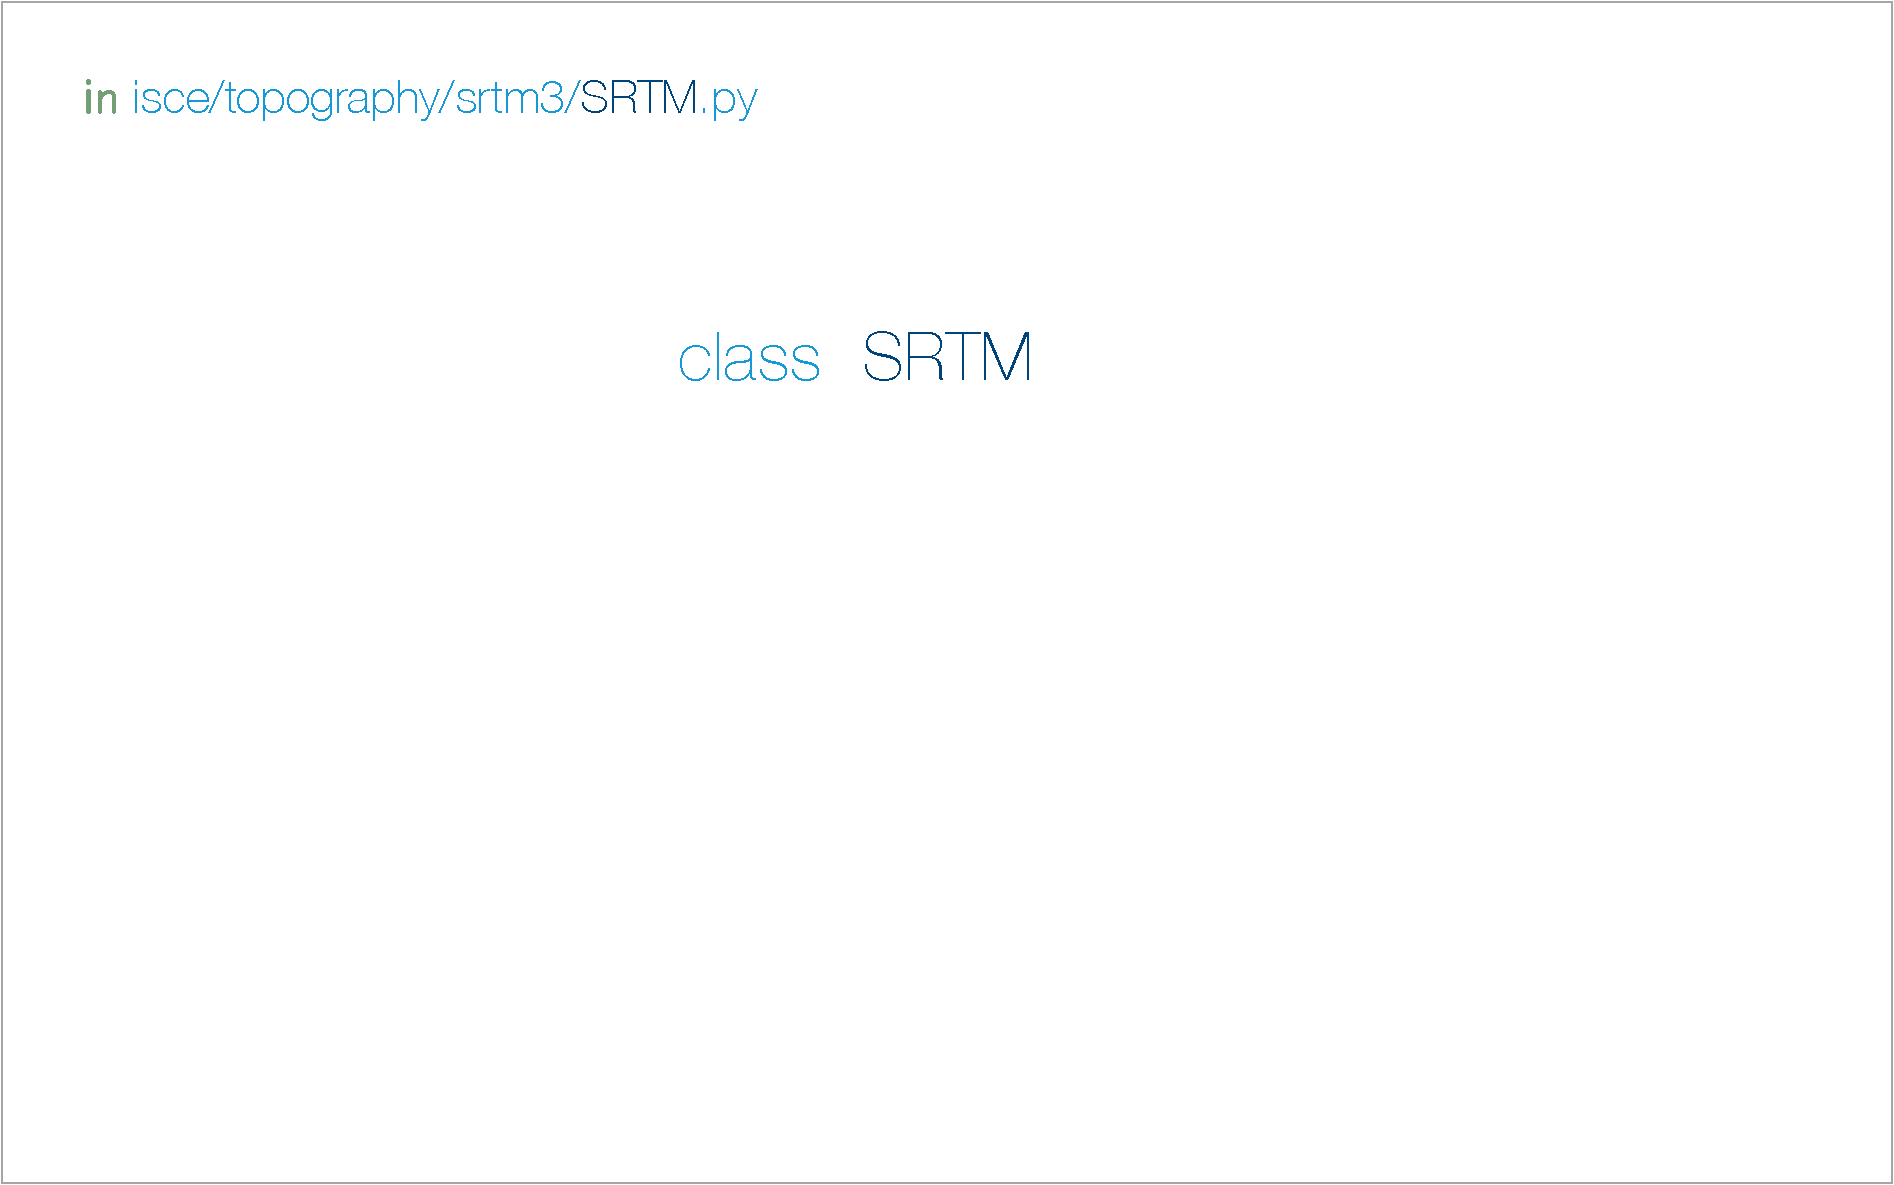
\includegraphics[width=0.9\textwidth]{component-package}
    \end{center}
  }
  \only<2->{
    \begin{center}
      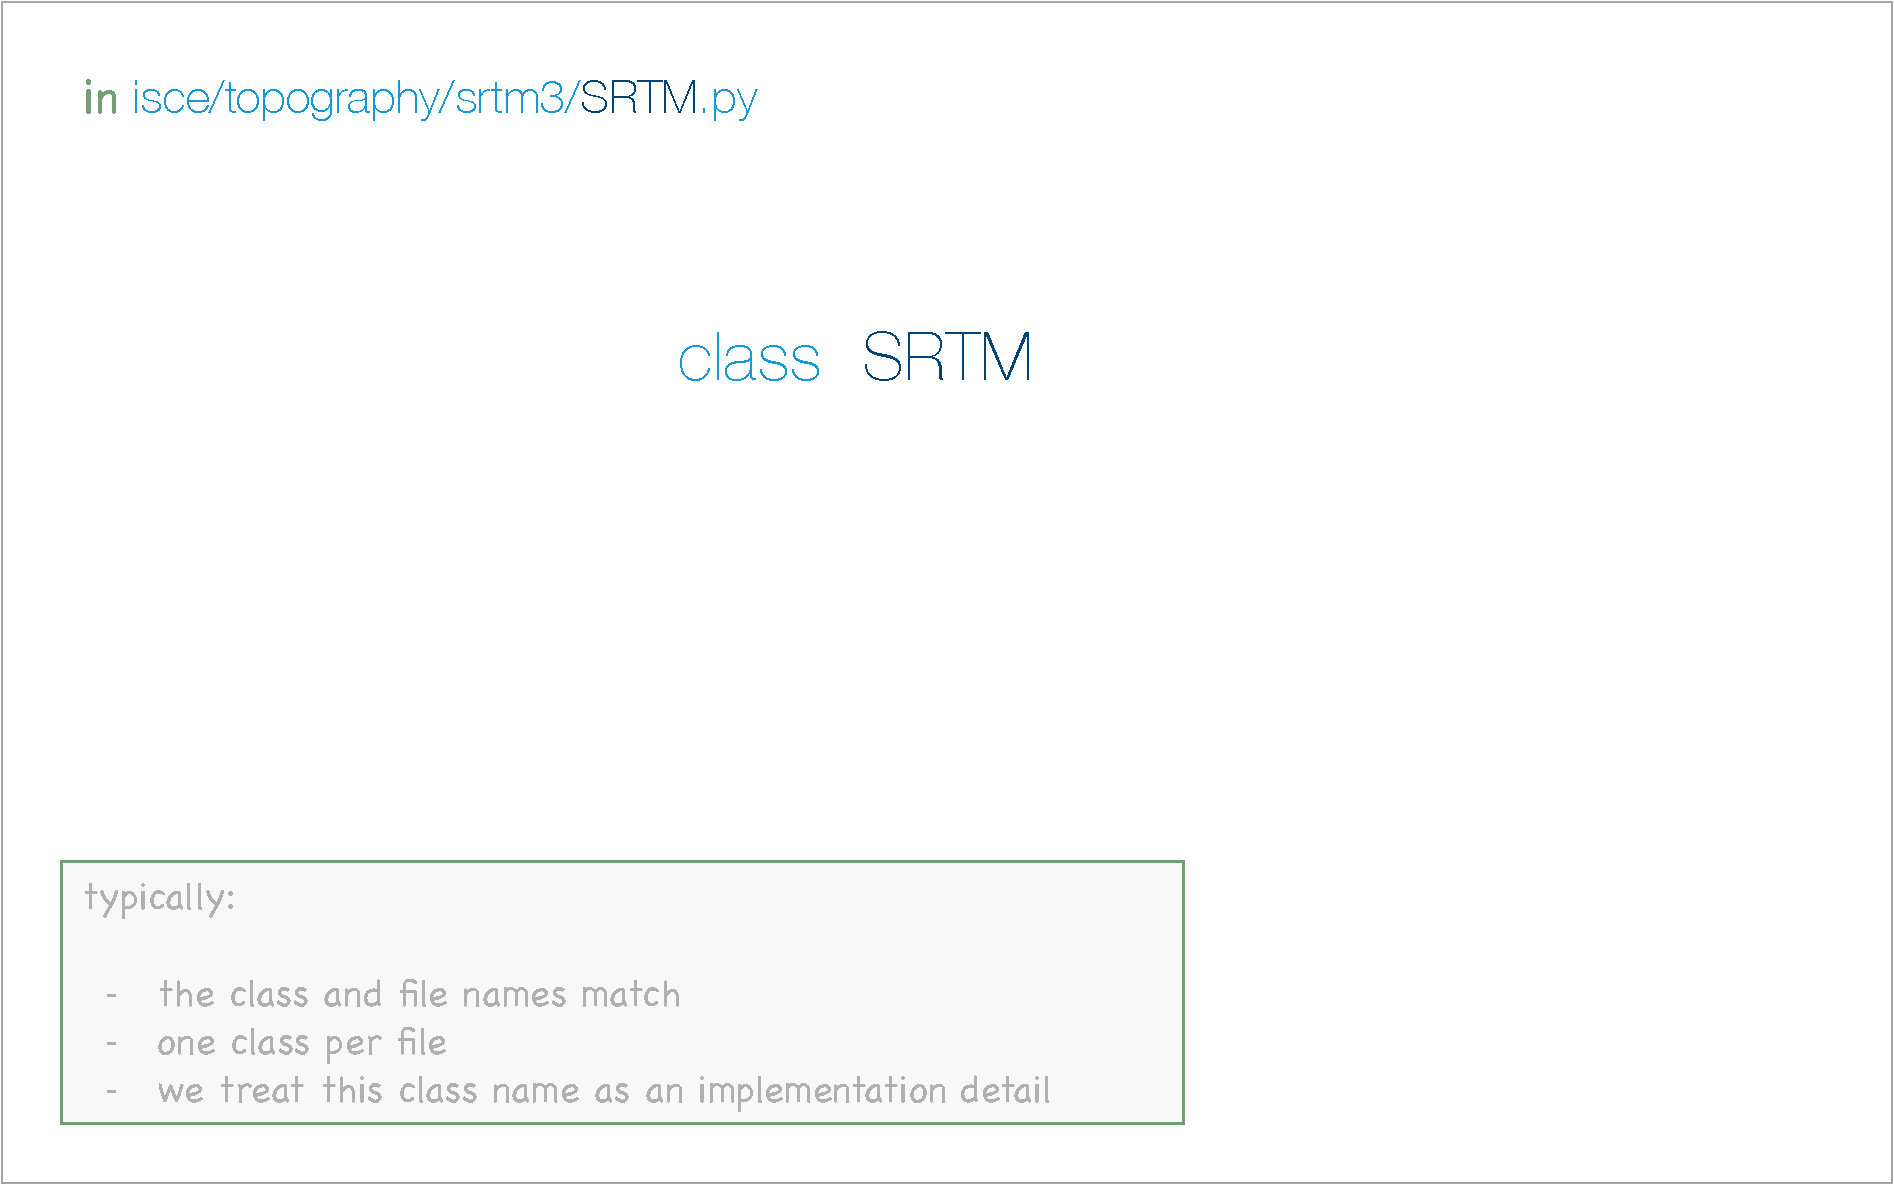
\includegraphics[width=0.9\textwidth]{component-package-explained}
    \end{center}
  }
%
\end{frame}

%-----------------------------------
\begin{frame}
%
  \frametitle{Turning classes into components}
%
  \only<1>{
    \begin{center}
      
\includegraphics[width=0.9\textwidth]{component-base}
    \end{center}
  }
  \only<2>{
    \begin{center}
      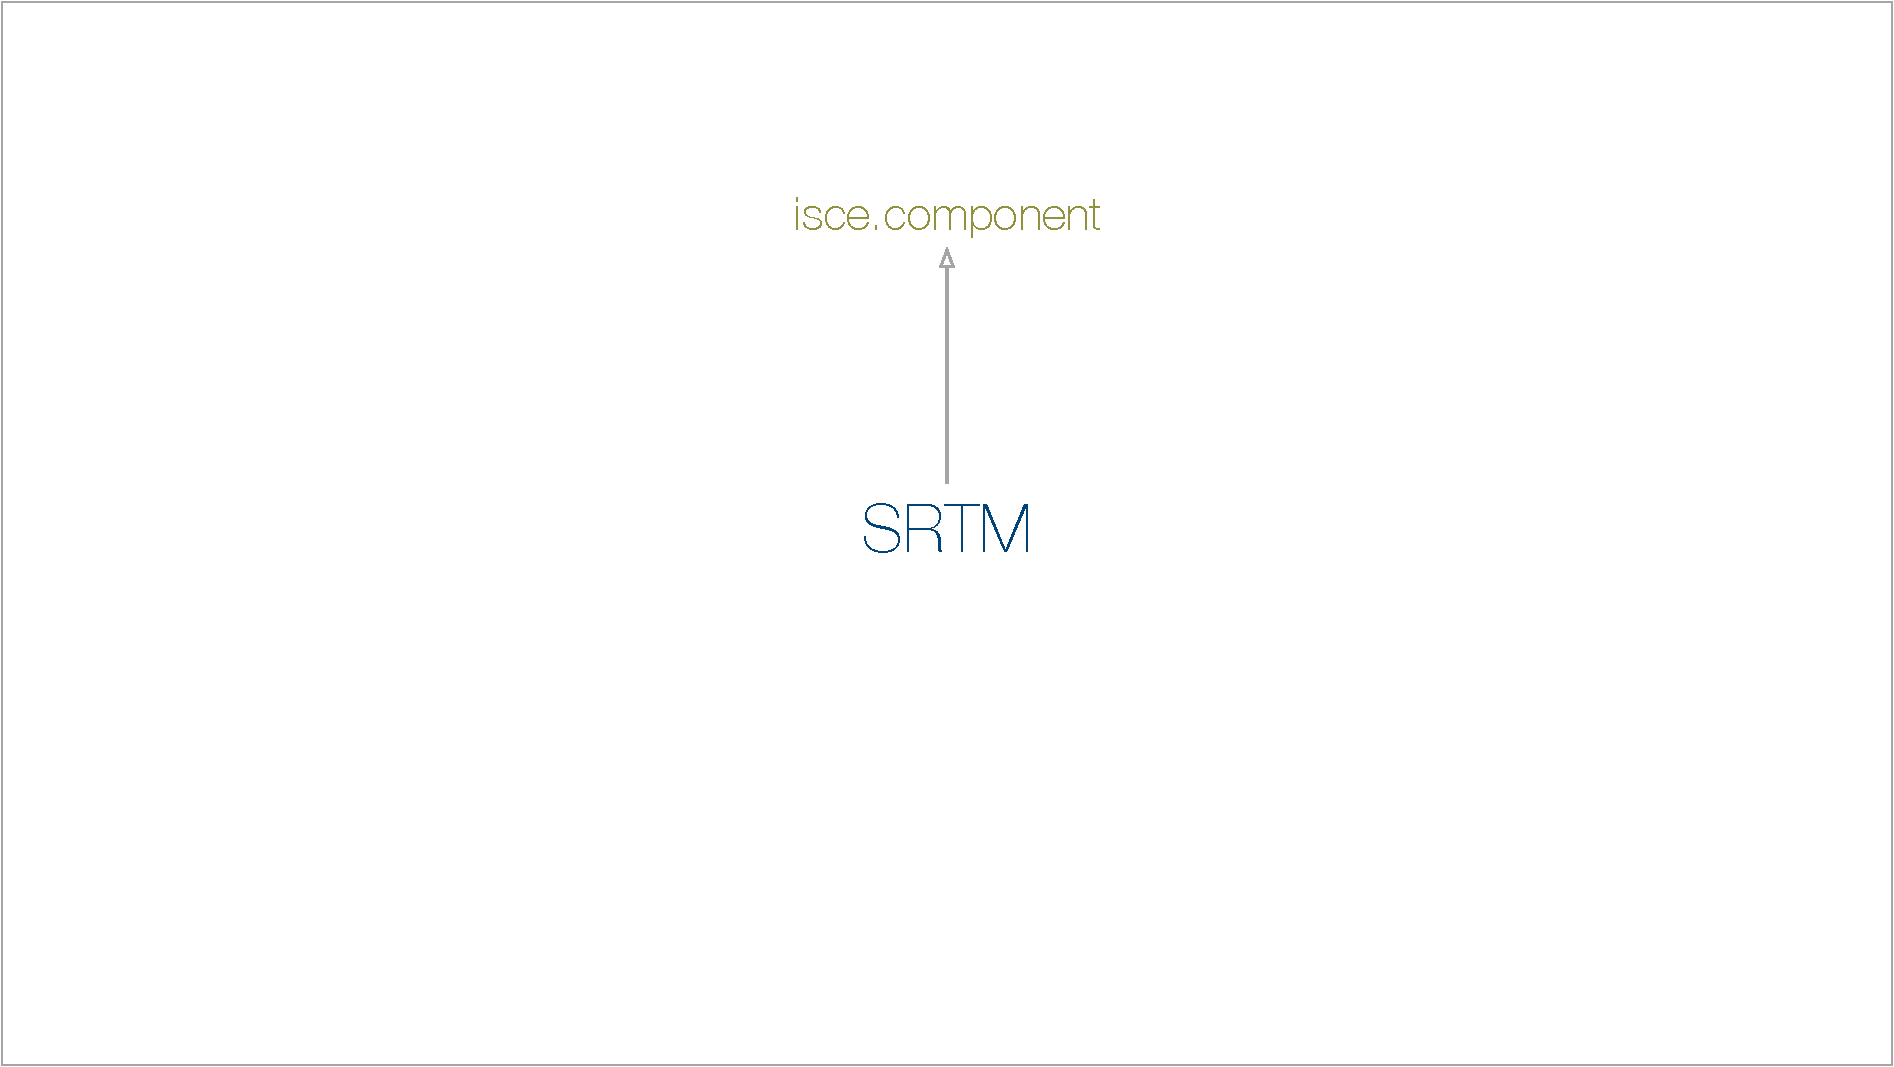
\includegraphics[width=0.9\textwidth]{component-inheritance}
    \end{center}
  }
  \only<3>{
    \begin{center}
      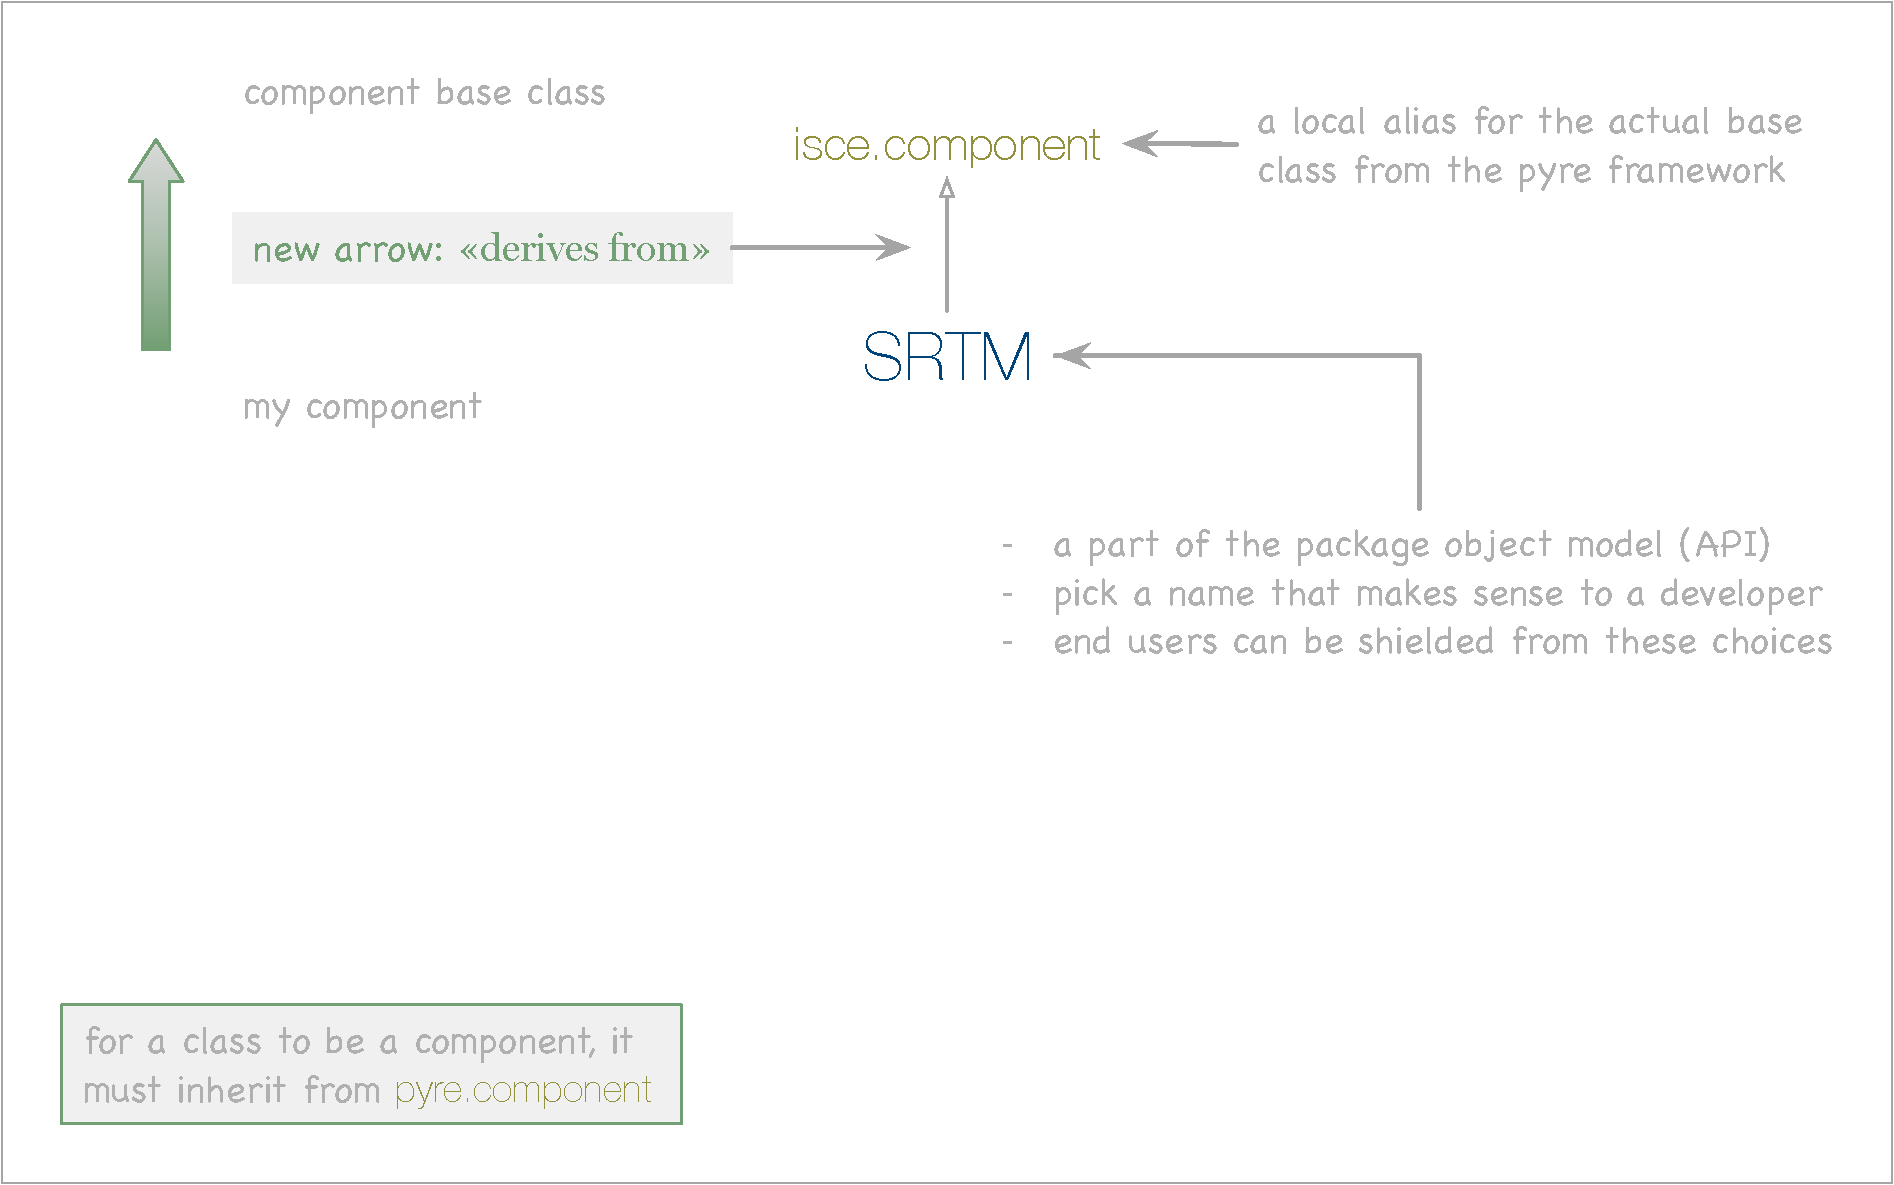
\includegraphics[width=0.9\textwidth]{component-inheritance-explained}
    \end{center}
  }
%
\end{frame}

%-----------------------------------
\begin{frame}[fragile]
%
  \frametitle{Component declaration}
%
  \vskip -3ex
  \begin{itemize}
%
  \item the instruction
    \begin{center}
      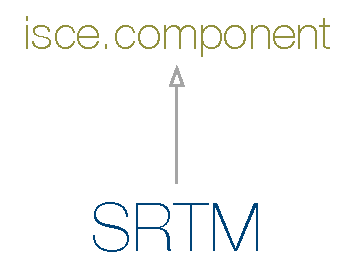
\includegraphics[height=10ex]{srtm-pedigree}
    \end{center}
%
  \item implies that instead of
%
    \begin{ipython}[gobble=6]{}
      class SRTM:
          """
          Access the SRTM data archive to download tiles and produce
          a digital elevation model for a specified region of interest
          """
    \end{ipython}
%
  \item we have to import the \isce\ package and derive from \pyrebuiltin{isce.component}:
    \begin{ipython}[gobble=6]{}
      # support
      import isce

      # the srtm component
      class SRTM(isce.component):
          """
          Access the SRTM data archive to download tiles and produce
          a digital elevation model for a specified region of interest
          """
    \end{ipython}
%
  \end{itemize}
%
\end{frame}

% --------------------------------------
\subsection{properties}

% properties
\begin{frame}[fragile]
%
  \frametitle{Specifying the tile resolution}
  \vskip -3ex
%
  \begin{itemize}
%
  \item version 3 \srtm\ tiles come in two resolutions; enable the user to choose
%
    \begin{ipython}[firstnumber=4, gobble=6]{}
      # the srtm component
      class SRTM(isce.component):
          """
          Access the SRTM data archive to download tiles and produce
          a digital elevation model for a specified region of interest
          """

          # user configurable state
          resolution = 1 # arc seconds per pixel
    \end{ipython}
%
  \item how do we read the value of \trait{resolution} from a configuration file?
%
    \begin{ipfg}{}
      srtm:
          resolution = 1 ; arc seconds per pixel
    \end{ipfg}
%
    or, equivalently, from the command line of some driver script?
%
    \begin{ish}{}
      dem.py --srtm.resolution=1
    \end{ish}
%
  \item there are two ingredients missing:
    \begin{itemize}
    \item \trait{resolution} must become a \emph{property} of \component{SRTM}, i.e.~the
      component register it as an attribute managed by the framework
    \item \component{SRTM} and its instances need \emph{names} so the user can refer to them
      from the user interface
    \end{itemize}
%
  \end{itemize}
%
\end{frame}

% --------------------------------------
% properties
\begin{frame}
%
  \frametitle{Components have properties}
%
  \only<1>{
    \begin{center}
      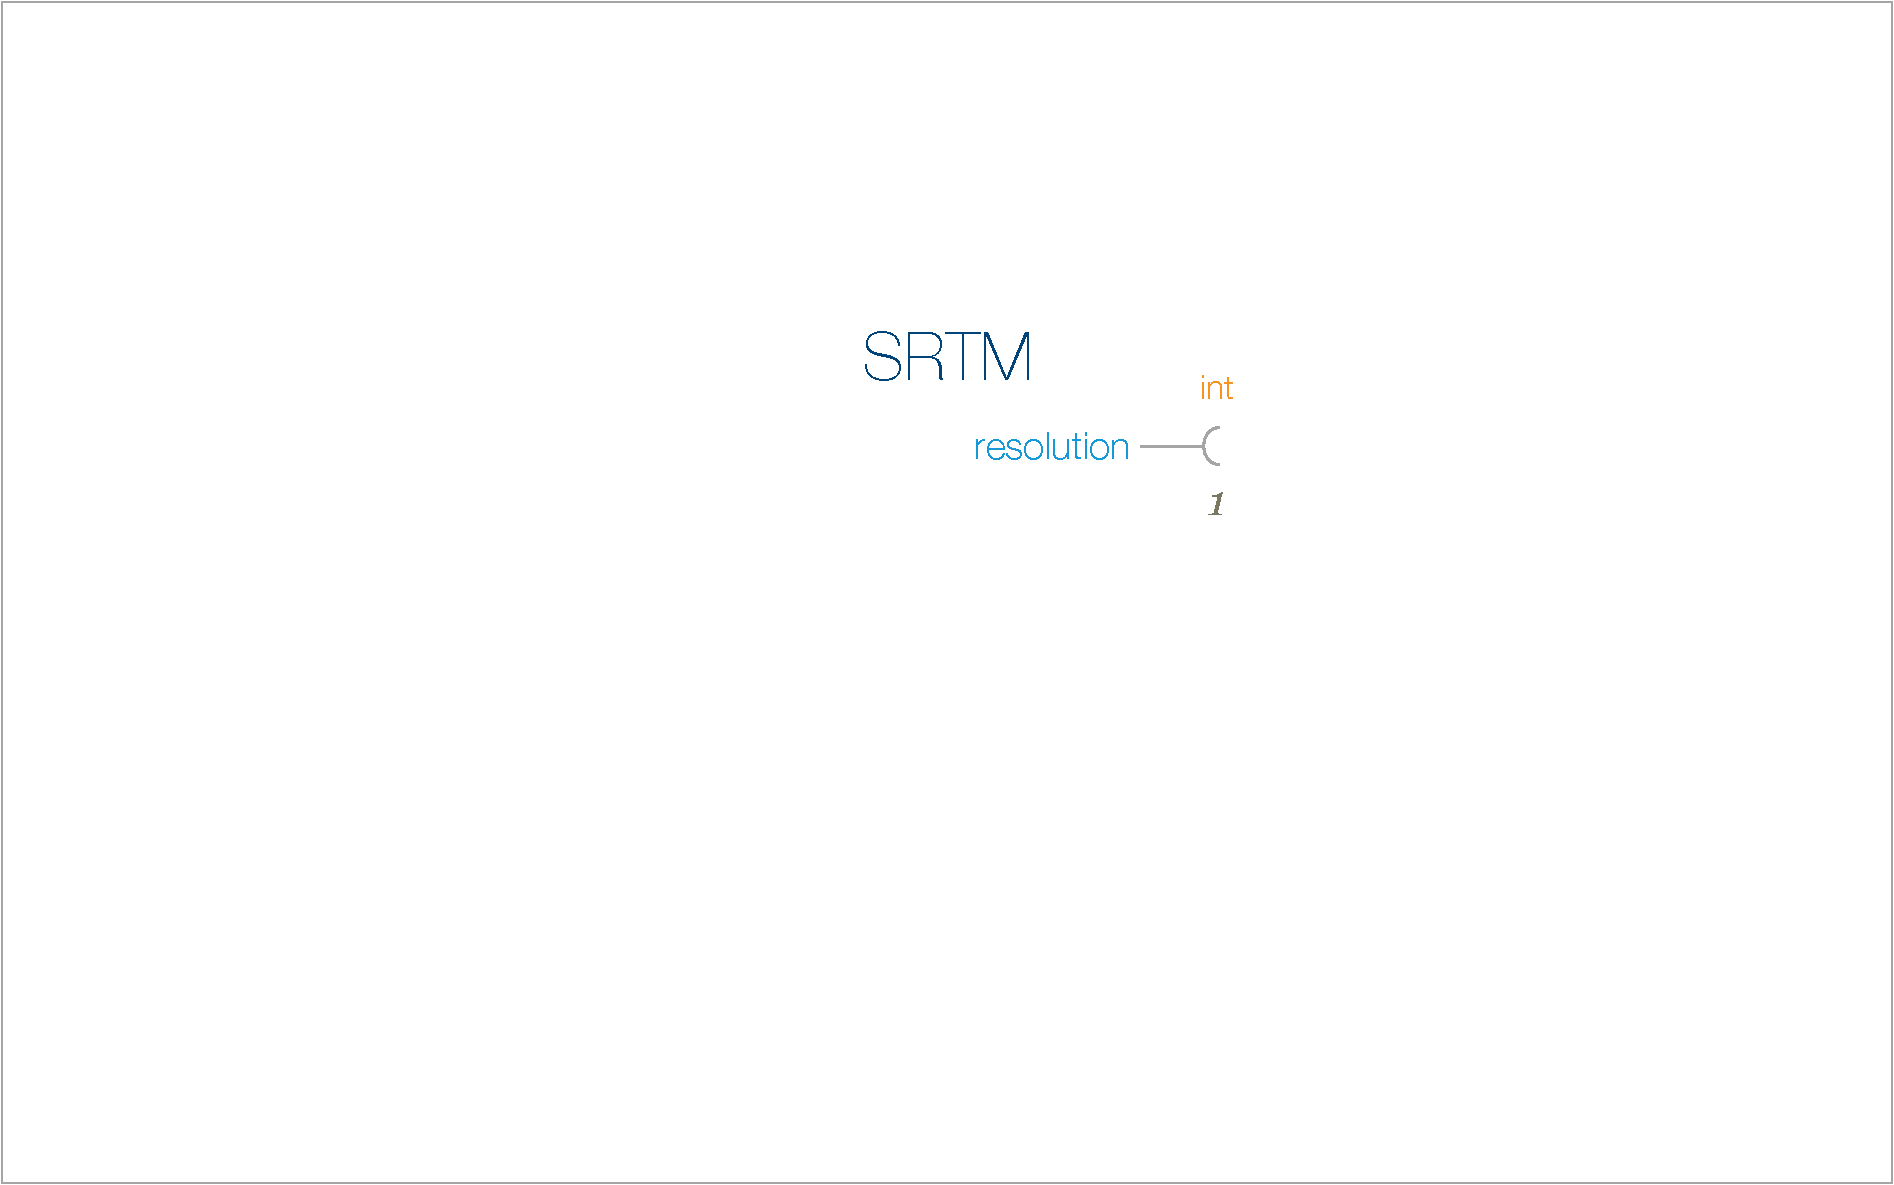
\includegraphics[width=0.9\textwidth]{component-properties}
    \end{center}
  }
  \only<2->{
    \begin{center}
      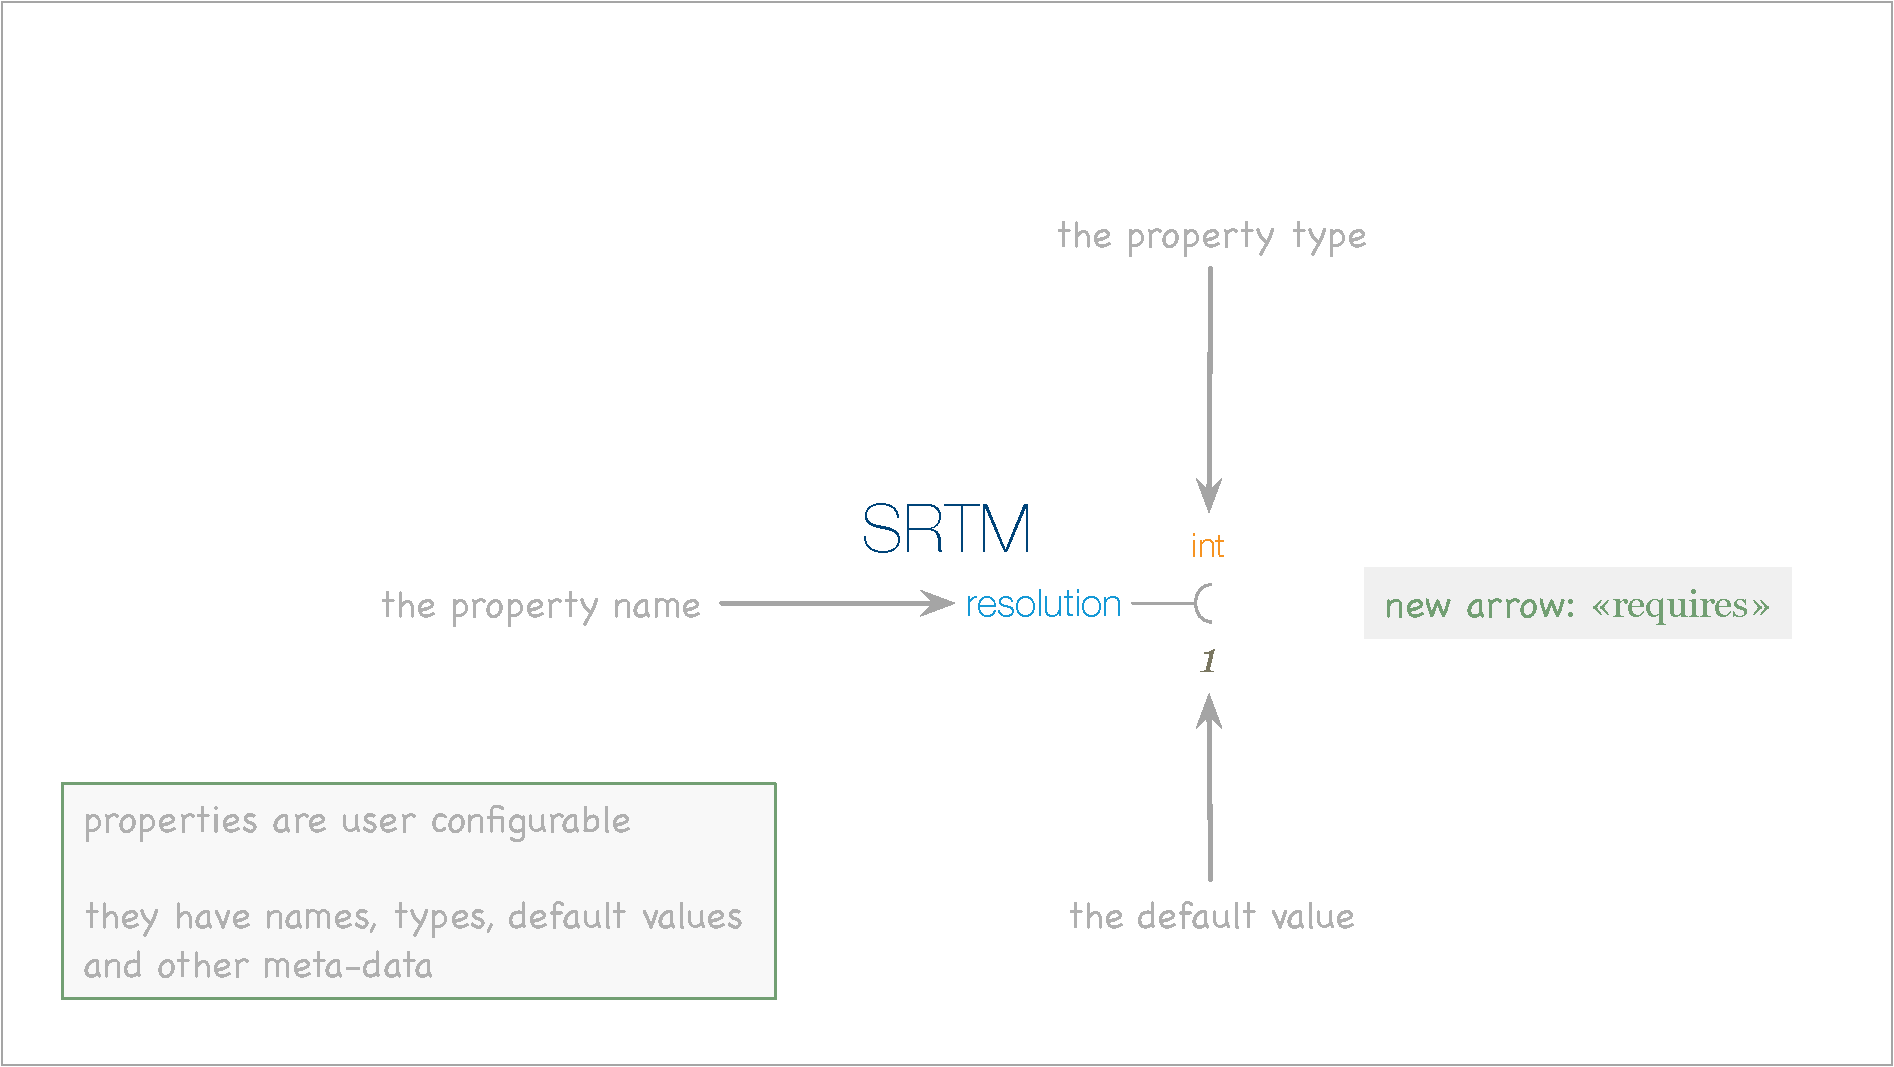
\includegraphics[width=0.9\textwidth]{component-properties-explained}
    \end{center}
  }
%
\end{frame}

% --------------------------------------
\begin{frame}[fragile]
%
  \frametitle{Property declarations}
%
  \vskip -4ex
  \begin{itemize}
%
  \item the instruction
%
    \begin{center}
      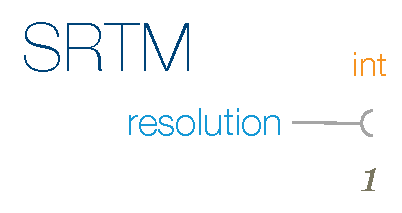
\includegraphics[height=10ex]{srtm-resolution}
    \end{center}
%
  \item implies the following modification to the \component{SRTM} declaration:
%
    \begin{ipython}[firstnumber=4, gobble=6]{}
      # the srtm component
      class SRTM(isce.component):
          """
          Access the SRTM data archive to download tiles and produce
          a digital elevation model for a specified region of interest
          """

          # user configurable state
          resolution = isce.properties.int(default=1)
          resolution.doc = 'the tile resolution in arc seconds per pixel'
    \end{ipython}
%
  \item why bother specifying the type of component properties?
    \begin{itemize}
    \item command line, configuration files, dialog boxes, web pages: they all gather
      information from the user as strings
    \item we need \emph{meta-data} so we can convert from strings to the intended object
    \end{itemize}
%
  \end{itemize}
%
\end{frame}

% --------------------------------------
\begin{frame}
%
  \frametitle{Properties}
%
  \vskip -2ex
  \begin{itemize}
%
  \item properties make sense for both classes and instances
    \begin{itemize}
    \item the class holds the default value that gets used in case the component instance does
      not have explicit configuration
    \item each instance gets its own private value when it gets configured
    \item the behavior is identical to regular python attributes
    \end{itemize}
%
  \item there is support for the following \emph{schemata}
    \begin{itemize}
    \item simple types: \basictype{bool}, \basictype{int}, \basictype{float},
      \basictype{decimal}, \basictype{fraction}, \basictype{str}
    \item containers: \basictype{tuple}, \basictype{list}, \basictype{set}, \schema{array}
    \item higher level: \basictype{date}, \schema{path}, \schema{uri}, \basictype{time},
      \schema{istream}, \schema{ostream}, \schema{inet}
    \item units: \schema{dimensional}
    \item composites: \schema{strings}, \schema{paths}, \schema{uris}
    \item easy enough to implement your own; the requirements are very simple
    \end{itemize}
%
  \item meta-data:
    \begin{itemize}
    \item \identifier{doc} and \identifier{tip}: simple and short documentation strings
    \item \identifier{default}: the default value, in case the user doesn't supply one
    \item \identifier{aliases}: a set of alternate names for the property
    \item \identifier{converters}: a chain of preprocessors of the string representation
    \item \identifier{normalizers}: a chain of post-processors of the converted value
    \item \identifier{validators}: a tuple of predicates that get called to ensure the property
      value satisfies the specified constraints
    \item you can add your own; the framework passes them through to your component
    \end{itemize}
%
  \end{itemize}
%
\end{frame}

%-----------------------------------
% values
\begin{frame}[fragile]
%
  \frametitle{Specifying property values}
%
  \vskip -4ex
  \begin{itemize}
%
  \item the value \keyword{None} is special: it means a property is uninitialized
    \begin{itemize}
    \item recognized as either the literal \keyword{None} or as the string \literal{'None'}
    \item it is a legal value for any trait
    \end{itemize}
%
  \item a property can be assigned a value that
    \begin{itemize}
    \item is already its native type
    \item can be converted to this native type by the trait schema
    \item can get through the validators without error
    \end{itemize}
%
  \item all property types recognize and process strings
    \begin{itemize}
    \item \basictype{bool} recognizes
      \literal{'true'}/\literal{'false'},
      \literal{'on'}/\literal{'off'},
      \literal{'yes'}/\literal{'no'} in any combination of upper case and lower case letters
    \item \basictype{int} and \basictype{float} evaluate simple expressions
    \item \basictype{date} and \basictype{time} let you specify a format string to use when parsing
      input
    \item \schema{istream} and \schema{ostream} interpret strings as filenames and open an
      associated stream
    \item \schema{path} and \schema{uri} have specialized parsers that convert strings to their
      internal representations of paths
    \end{itemize}
%
  \item string values may refer to other properties by name, so something like this could work
    \begin{ipython}[gobble=2]{}
      srtm.resolution = "3600 / {tile.width}"
    \end{ipython}
    arithmetic can be done in configuration files -- and the command line
%
  \end{itemize}
%
\end{frame}

%-----------------------------------
% containers
\begin{frame}[fragile]
%
  \frametitle{Containers}
%
  \vskip -4ex
  \begin{itemize}
%
  \item there are three basic container types: \basictype{tuple}, \basictype{list} and
    \basictype{set}
%
  \item you must supply the type of the contained item so conversions can happen correctly
%
  \item given the component declaration
    \begin{ipython}[gobble=4]{}
      class Band(isce.component):
          """
          An illustration of property containers
          """

          names = isce.properties.tuple(schema=isce.properties.str())
          names.default = 'john, paul, george, ringo'
    \end{ipython}
%
    the code fragment
    \begin{ipython}[firstnumber=9, gobble=4]{}
      >>> beatles = Band(name='beatles') # more on instantiating components later on
      >>> print(beatles.names)
    \end{ipython}
%
    produces
%
    \begin{ipython}[firstnumber=11, gobble=4]{}
      ['john', 'paul', 'george', 'ringo']
      >>>
    \end{ipython}
%
    more sophisticated -- and realistic -- examples coming up
%
  \item \schema{array} passes its values through \function{eval}; it accepts any expression that
    evaluates into an iterable without doing much error checking
%
  \end{itemize}
%
\end{frame}

% --------------------------------------
% units
\begin{frame}[fragile]
%
  \frametitle{Units}
%
  \vskip -3ex
  \begin{itemize}
%
  \item \schema{dimensional} properties have units
%
  \item the low level support is in \package{isce.units}
    \begin{itemize}
    \item full support for all SI base and derived units
    \item all common abbreviations and names from alternative systems of units
    \item correct arithmetic; proper handling of functions from \package{math}
    \item distributive over containers: \literal{[1,2,3]*m -> [1*m,2*m,3*m]}
    \end{itemize}
%
  \item consider
    \begin{ipython}[gobble=6]{}
      from math import cos
      from isce.units.SI import meter, second, radian

      A = 2.5 * meter
      t = 1.5 * second
      ω = 4.2 * radian/second

      x = A * cos(ω * t)
     \end{ipython}
%
   \item an exception is raised if the units in the argument to \function{cos} do not cancel,
     leaving a pure \basictype{float} behind; \identifier{x} has dimensions of meters
%
   \item there is some control over the printing value
%
    \begin{ipython}[firstnumber=9, gobble=6]{}
      pretty = '{:value=.2f, base={scale}, label=cm}'.format(x, scale=meter/100)
    \end{ipython}
%
  \end{itemize}
%
\end{frame}

% --------------------------------------
% constraints
\begin{frame}[fragile]
%
  \frametitle{Constraints}
%
  \begin{itemize}
%
  \item there are only two valid values for \trait{resolution}
%
    \begin{ipython}[firstnumber=4, gobble=6]{}
      # the srtm component
      class SRTM(isce.component):
          """
          Access the SRTM data archive to download tiles and produce
          a digital elevation model for a specified region of interest
          """

          # user configurable state
          resolution = isce.properties.int(default=1)
          resolution.doc = 'the tile resolution in arc seconds per pixel'
          resolution.validators = isce.constraints.isMember(1, 3)
    \end{ipython}
%
    any attempt to set \trait{resolution} to a value other than $1$ or $3$ will raise an
    exception
%
  \item the full list of primitives are
    \begin{itemize}
    \item \constraint{isEqual}, \constraint{isGreater},
      \constraint{isGreaterEqual},\constraint{isLess}, \constraint{isLessEqual}
    \item \constraint{isPositive}, \constraint{isNegative}, \constraint{isBetween}
    \item \constraint{isMember}, \constraint{isSubset}, \constraint{isLike}
    \end{itemize}
%
  \item they can be combined using
    \begin{itemize}
    \item \constraint{isNot}
    \item \constraint{isAll}, \constraint{isAny}
    \end{itemize}
%
  \item easy to extend
%
  \end{itemize}
%
\end{frame}

%-----------------------------------

\begin{frame}[fragile]
%
  \frametitle{Specifying the region}
%
  \vskip -4ex
  \begin{itemize}
%
  \item let's add the \trait{region} requirement
%
    \begin{center}
      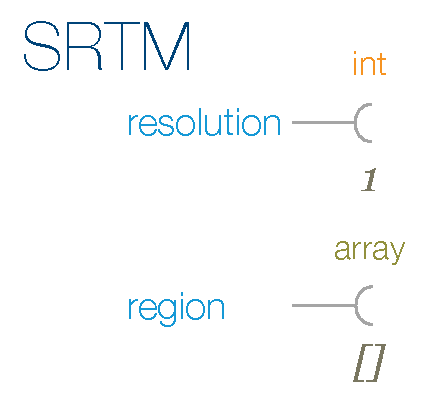
\includegraphics[height=15ex]{srtm-region}
    \end{center}
%
  \item the \component{SRTM} declaration becomes:
%
    \begin{ipython}[firstnumber=4, gobble=6]{}
      # the srtm component
      class SRTM(isce.component):
          """
          Access the SRTM data archive to download tiles and produce
          a digital elevation model for a specified region of interest
          """

          # user configurable state
          resolution = isce.properties.int(default=1)
          resolution.doc = 'the tile resolution in arc seconds per pixel'
          resolution.validators = isce.constraints.isMember(1, 3)

          region = isce.properties.array()
          region.doc = 'a cloud of (lat,lon) pairs'
    \end{ipython}
%
  \end{itemize}
%
\end{frame}

%-----------------------------------

\begin{frame}
%
  \frametitle{More notation}
  \vskip -3ex
%
  \begin{itemize}
%
  \item when we don't care to show the binding slots, here is a more compact alternative to the
    property declarations
%
    \begin{center}
      
\includegraphics[height=10ex]{srtm-properties-compact}
    \end{center}
%
%
  \item sometimes we need to communicate the values to which properties are bound
%
    \begin{center}
      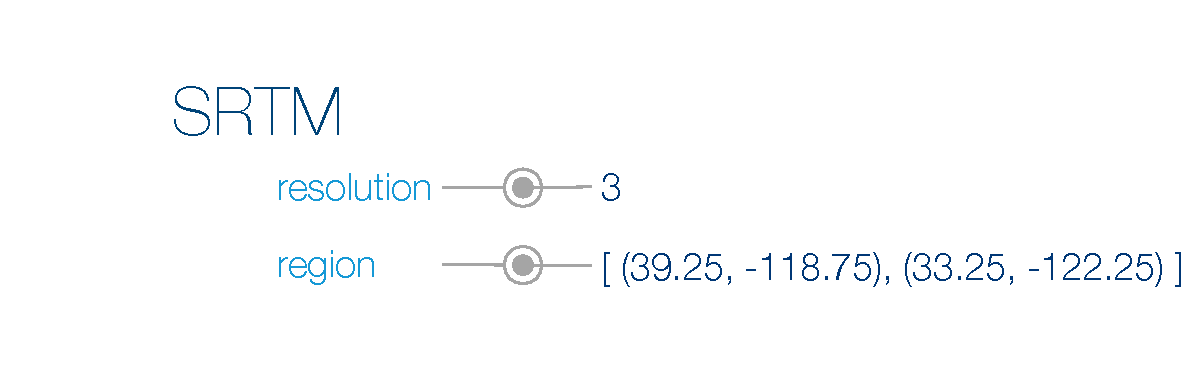
\includegraphics[height=10ex]{srtm-properties-bound}
    \end{center}
%
  \item when we don't need the connectors, we can be more compact
%
    \begin{center}
      
\includegraphics[height=10ex]{srtm-properties-bound-compact}
    \end{center}
%
  \end{itemize}
%
\end{frame}

%-----------------------------------
\subsection{names}
\begin{frame}[fragile]
%
  \frametitle{The names of things}
%
  \begin{itemize}
%
  \item in order to connect components to configurations, component authors and end
    users have to agree on the names of things
%
  \item classes already have names
    \begin{itemize}
    \item but the python runtime environment uses these for internal purposes
    \item not end-user friendly
    \end{itemize}
%
  \item python instances are not automatically assigned anything meaningful
    \begin{itemize}
    \item typically, their \function{id} is related to their location in memory
    \item not end-user friendly
    \item not persistent across program invocations
    \end{itemize}
%
  \item the current solution is to place the burden on the component developer to design
    rational namespaces that are meaningful and easy to remember
    \begin{itemize}
    \item admittedly, not an easy problem
    \item but forces some design issues to the forefront, so overall a good thing\texttrademark
    \end{itemize}
%
  \item all names are optional
    \begin{itemize}
    \item public versus private; for \pyre: end-user visible or not
    \item if an entity doesn't have a name, it's functional but not configurable
    \end{itemize}
%
  \item component instances may be given unique names during instantiation
%
  \item component classes may be given unique family names during declaration
%
  \item namespace management: components belong to packages
%
  \end{itemize}
%
\end{frame}

%-----------------------------------
\begin{frame}
%
  \frametitle{Public components and their instances}
%
    \only<1>{
      \begin{center}
        
\includegraphics[width=0.9\textwidth]{component-family}
      \end{center}
    }
    \only<2>{
      \begin{center}
        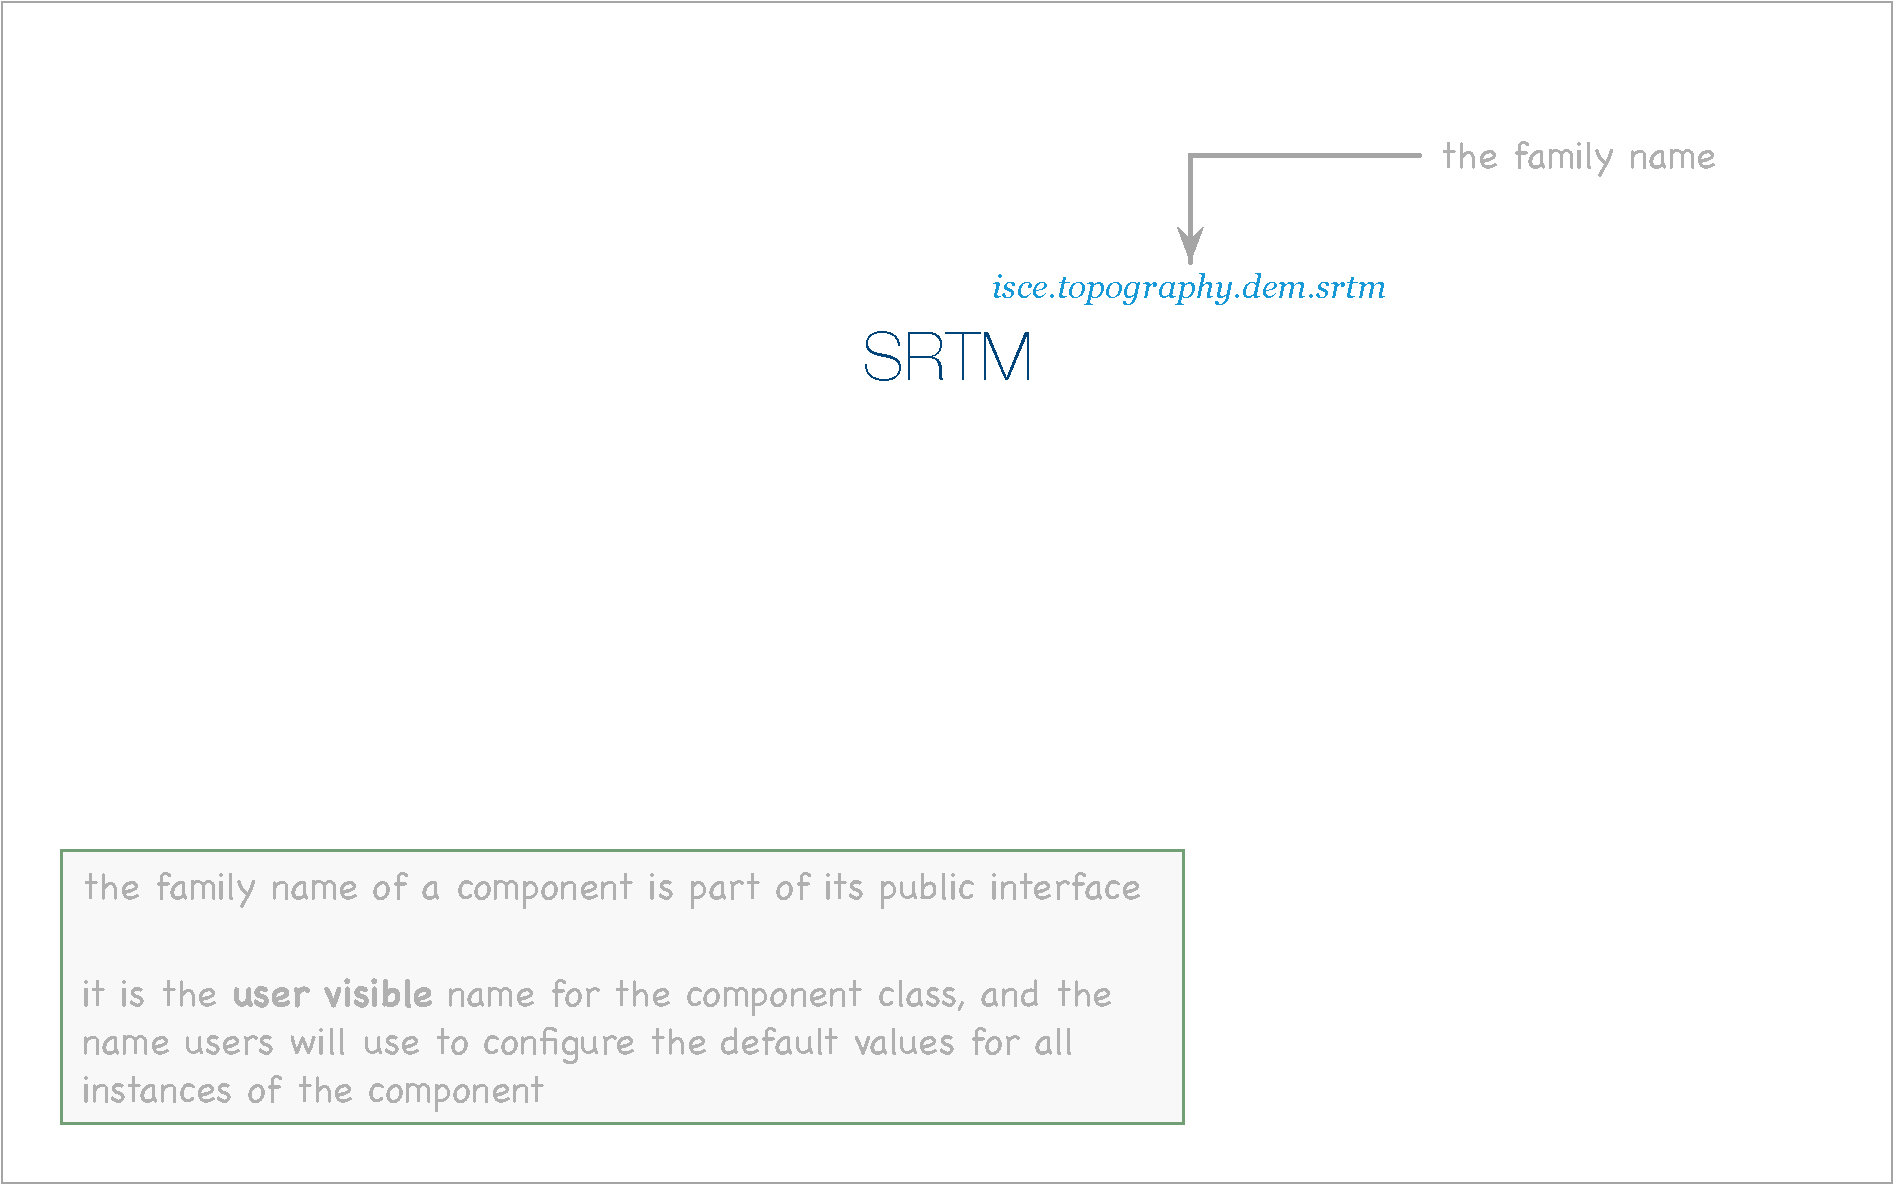
\includegraphics[width=0.9\textwidth]{component-family-explained}
      \end{center}
    }
    \only<3>{
      \begin{center}
        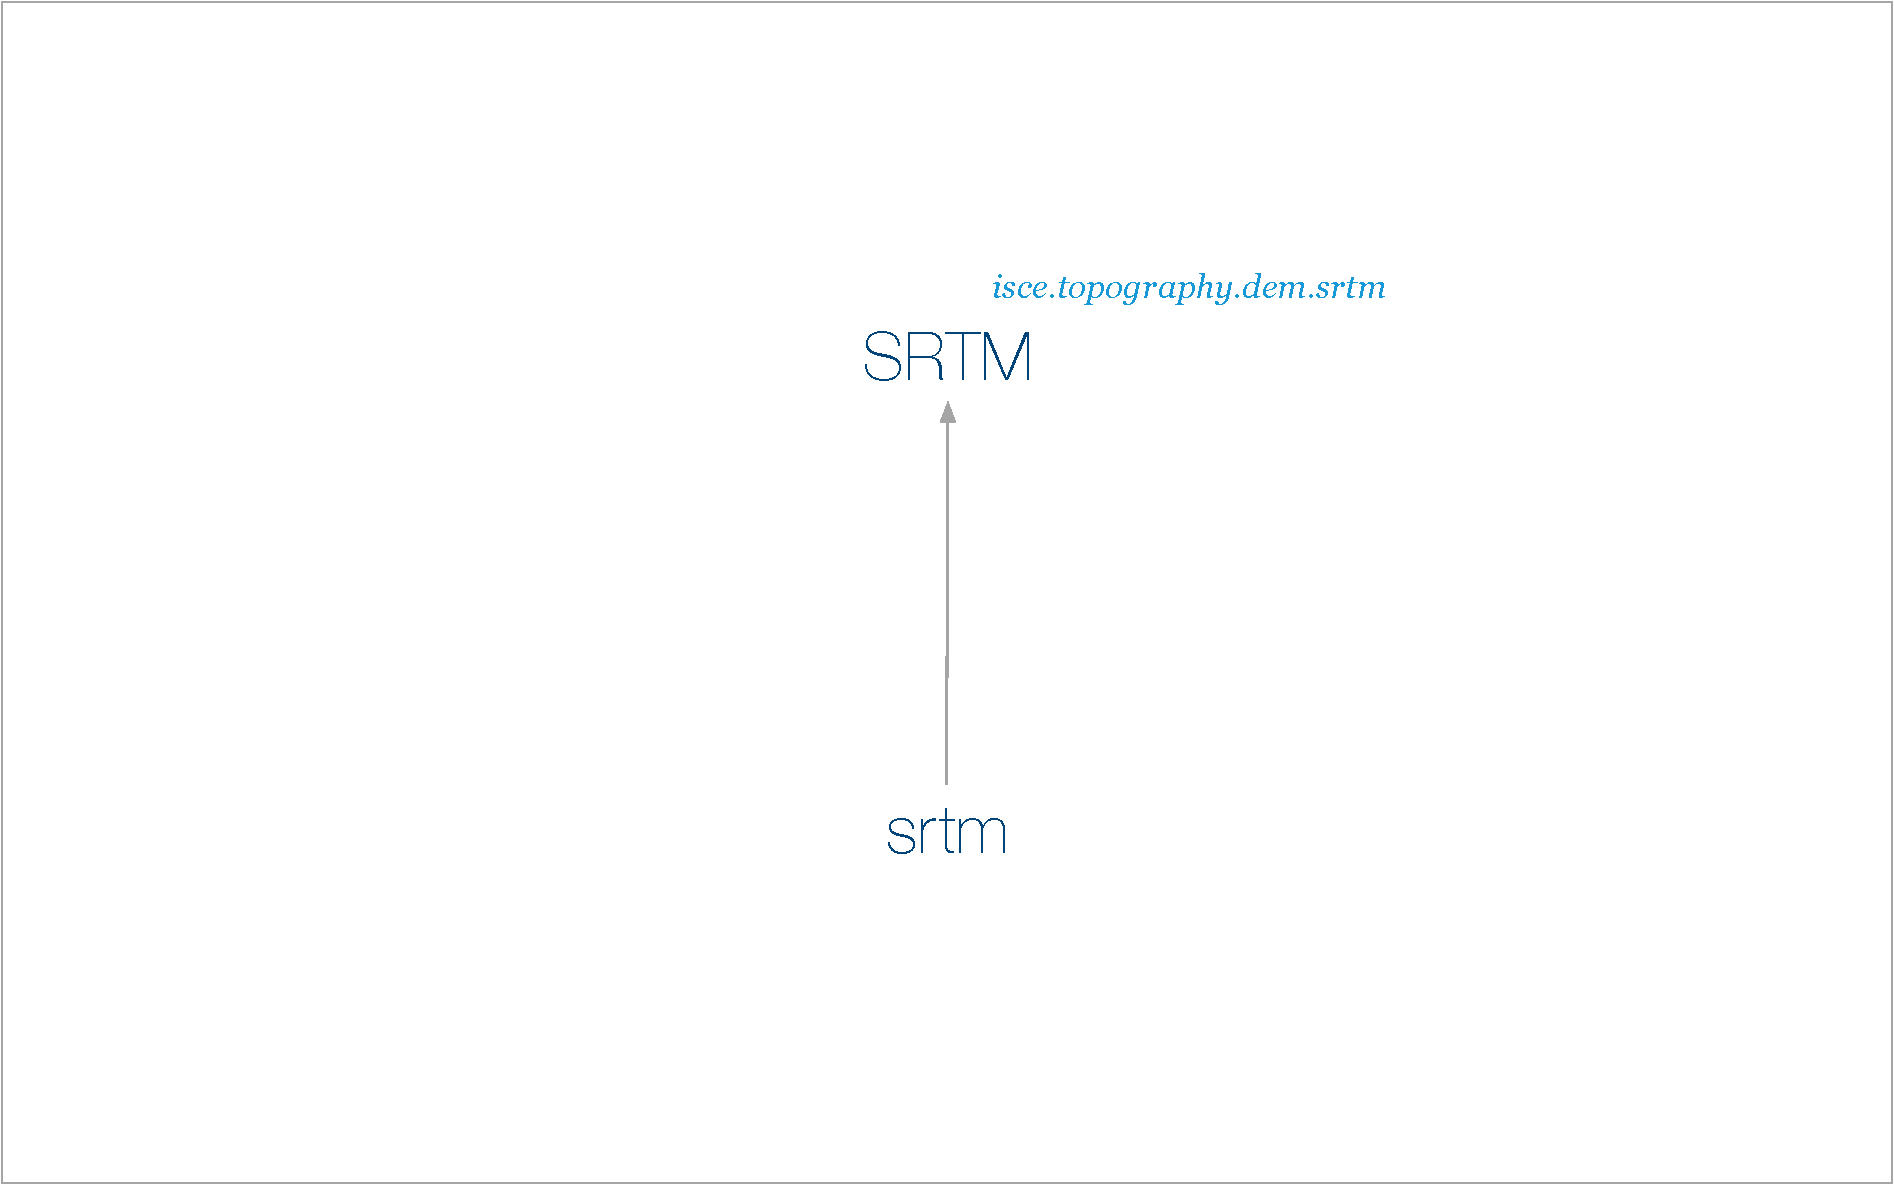
\includegraphics[width=0.9\textwidth]{component-instance}
      \end{center}
    }
    \only<4>{
      \begin{center}
        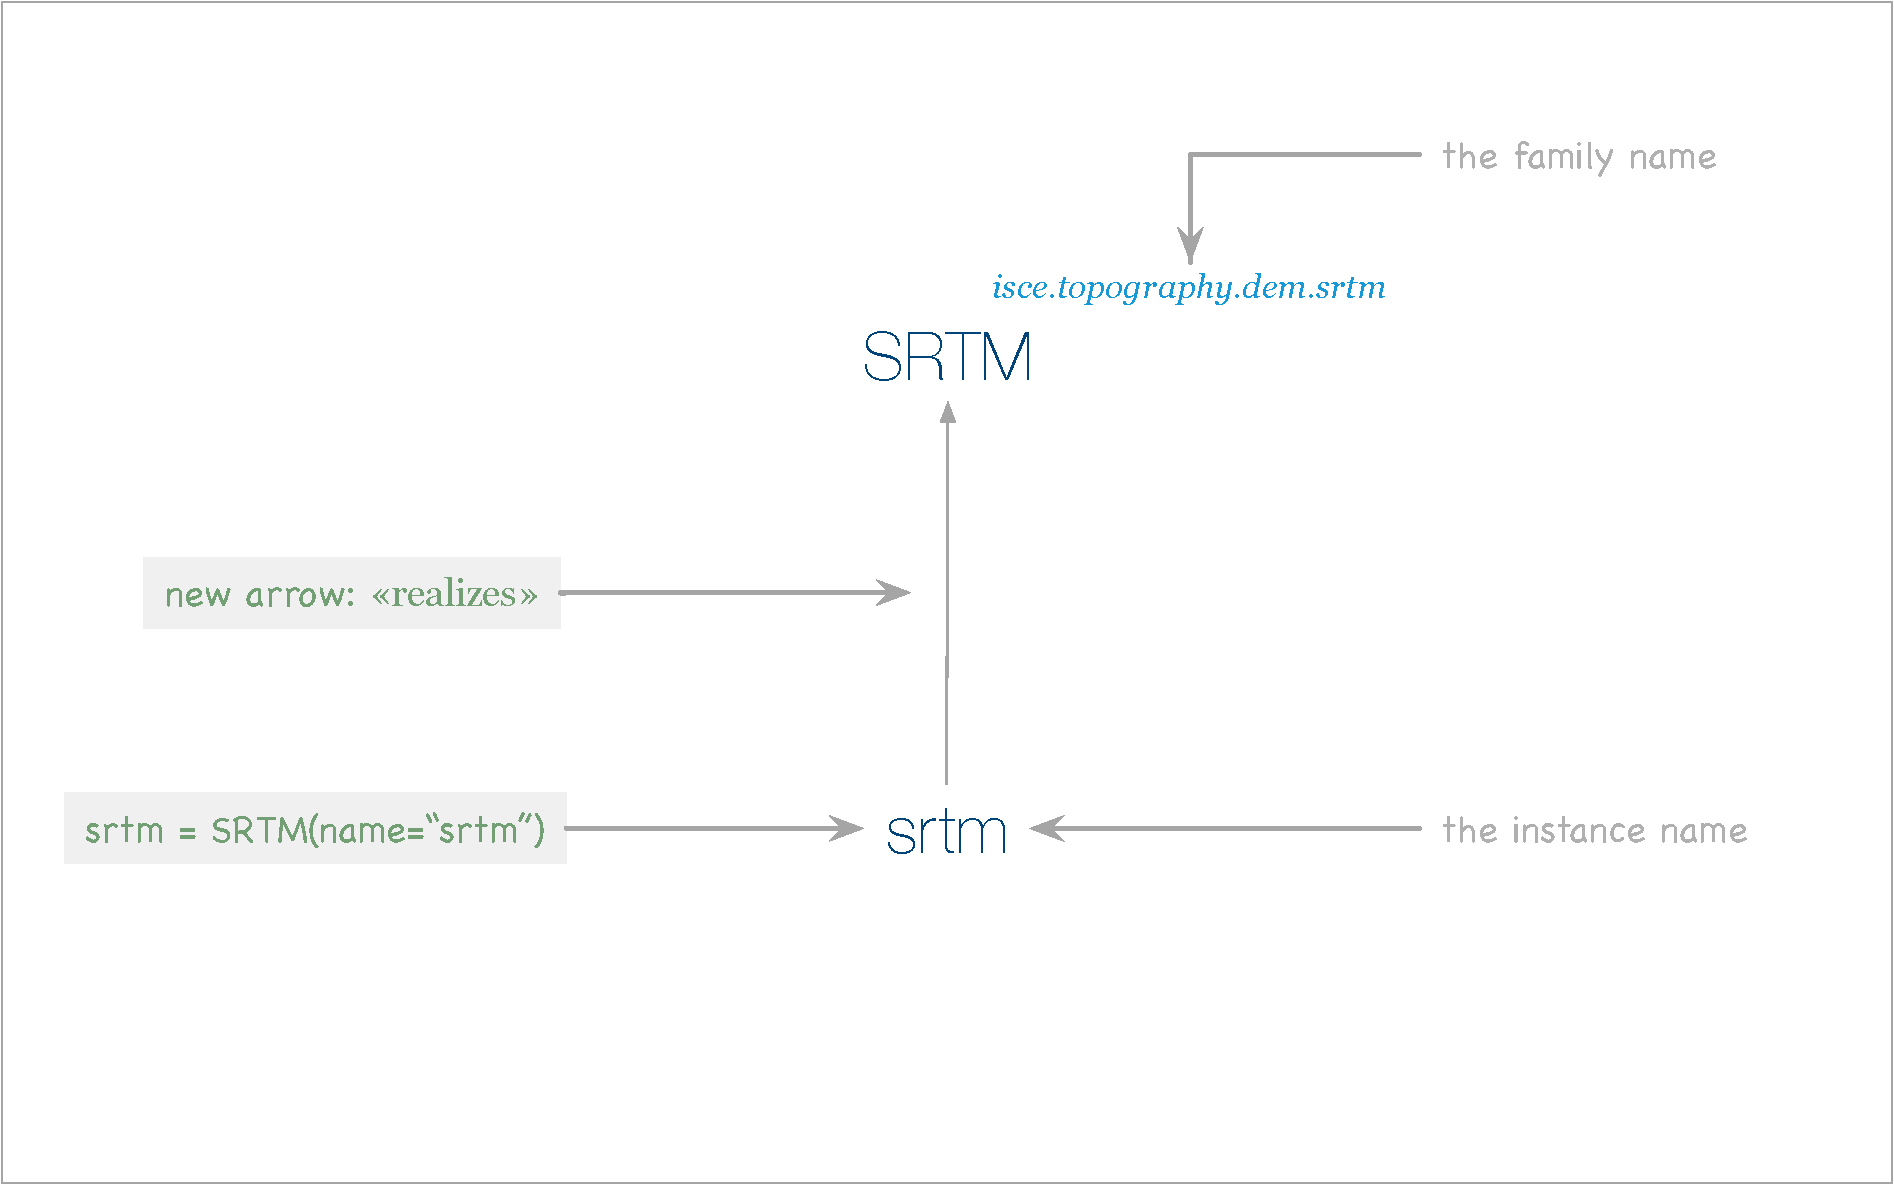
\includegraphics[width=0.9\textwidth]{component-instance-explained}
      \end{center}
    }
    \only<5>{
      \begin{center}
        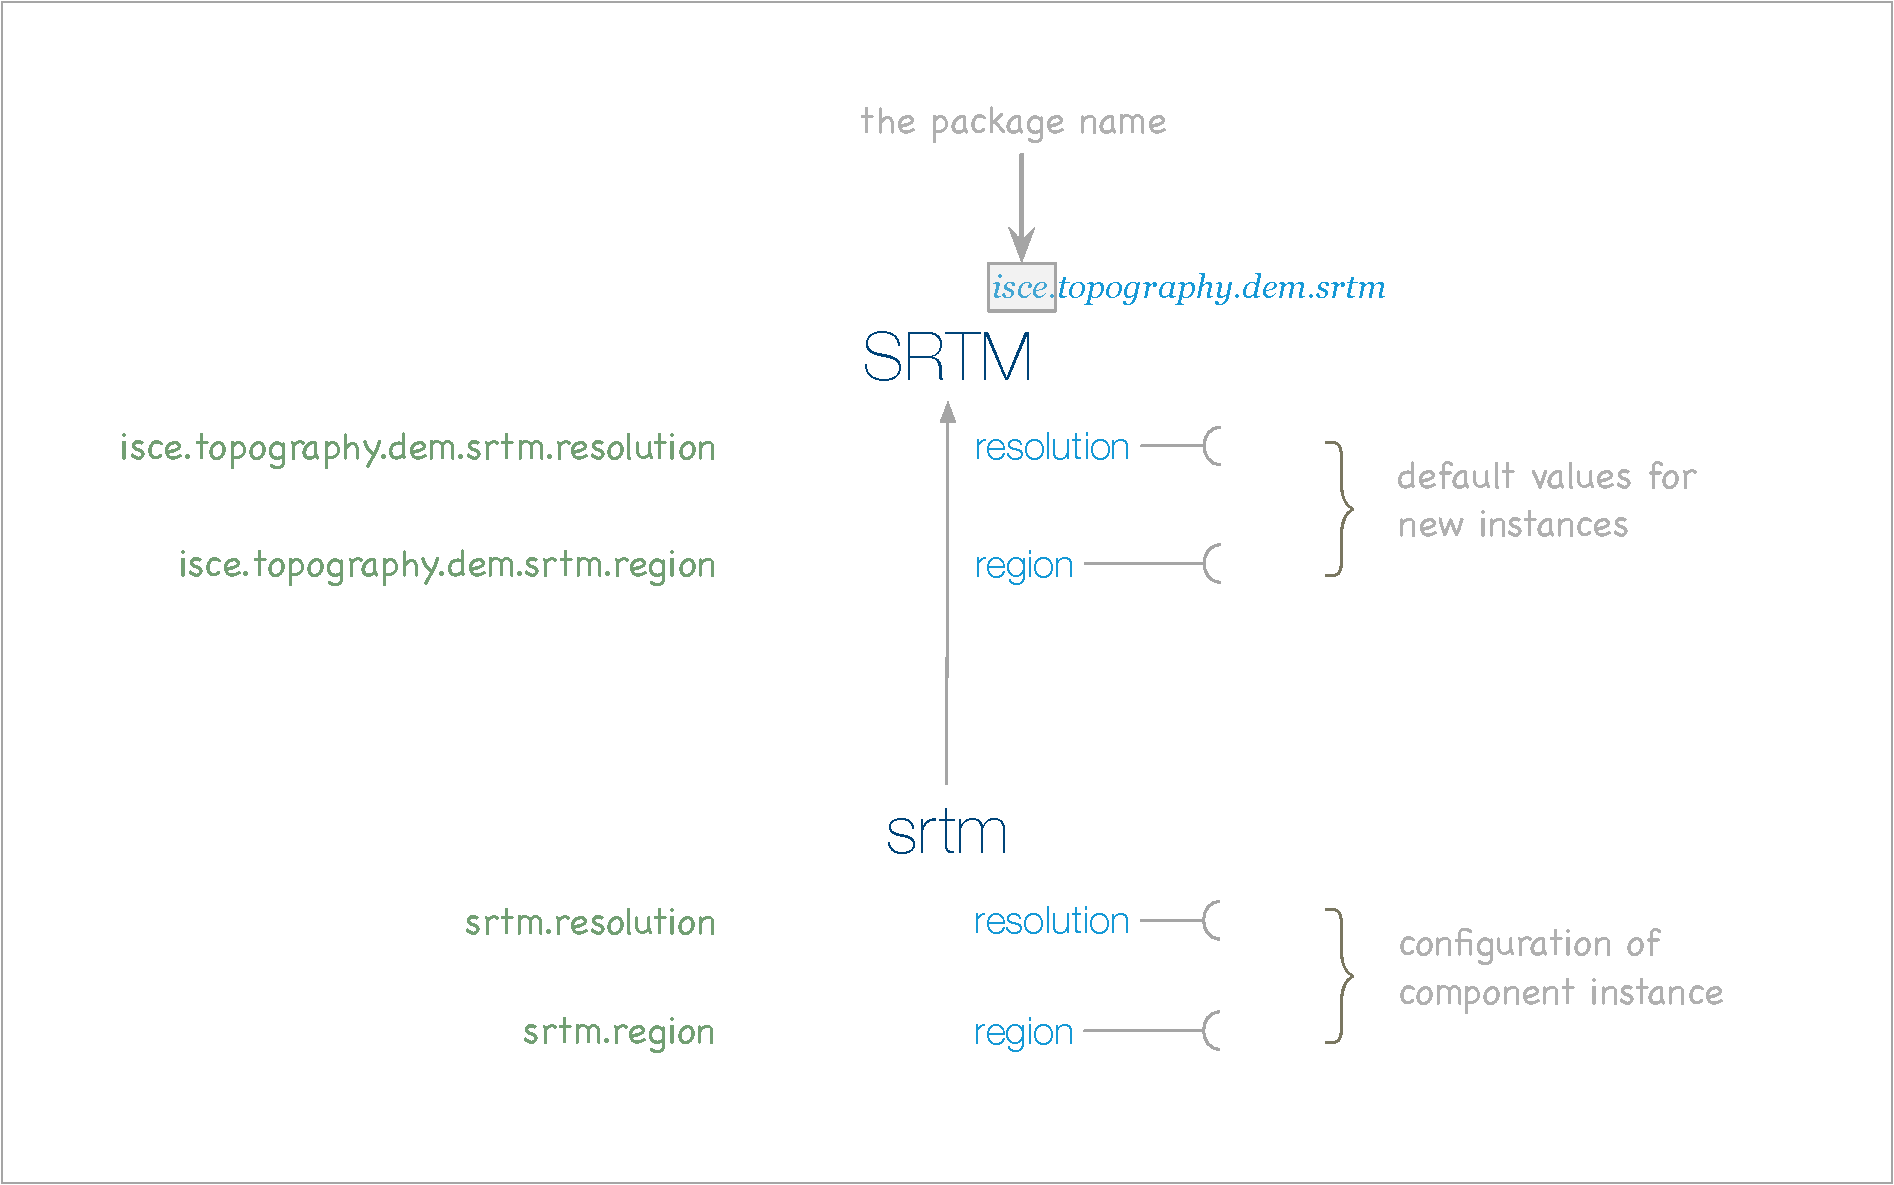
\includegraphics[width=0.9\textwidth]{component-config}
      \end{center}
    }
    \only<6>{
      \begin{center}
        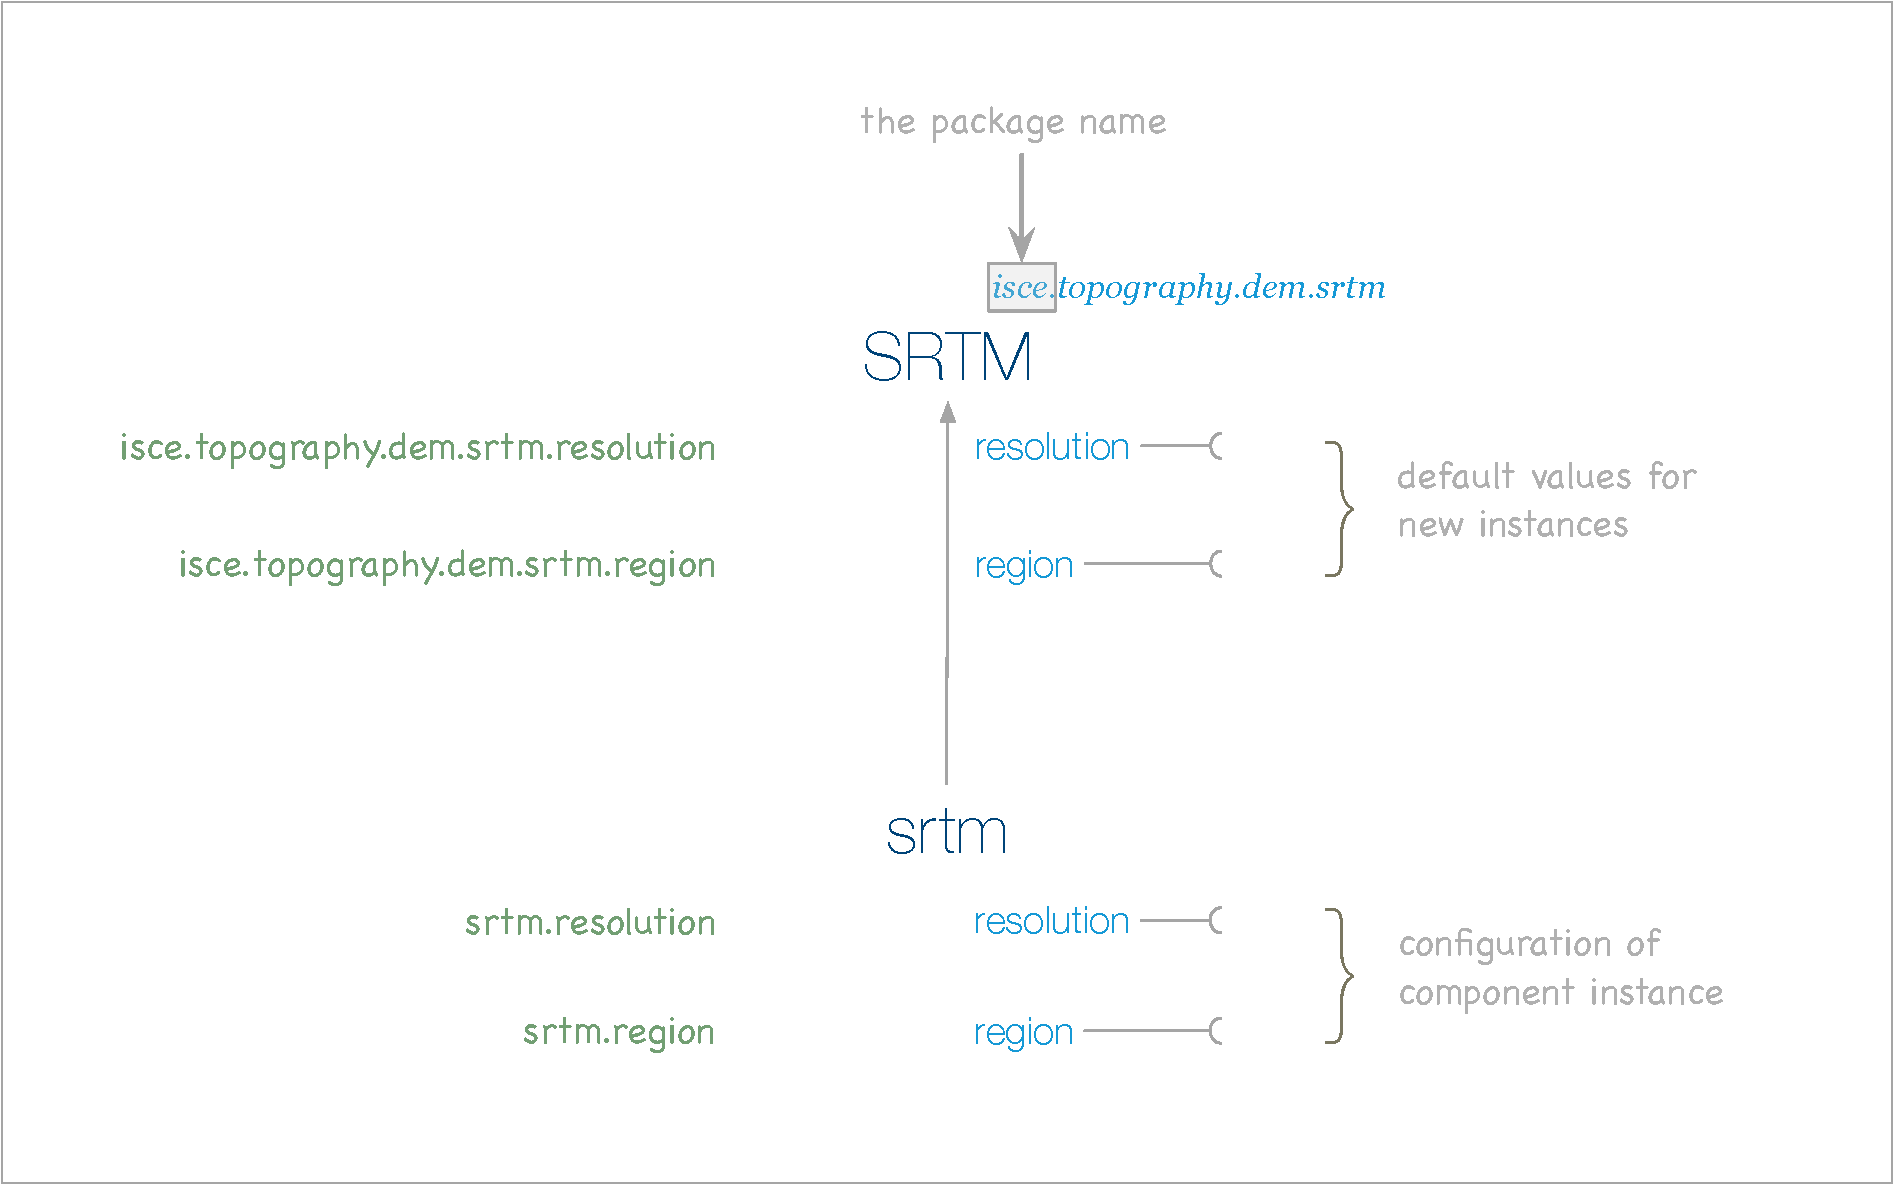
\includegraphics[width=0.9\textwidth]{component-config-explained}
      \end{center}
    }
%
\end{frame}

% --------------------------------------
\begin{frame}[fragile]
%
  \frametitle{Adding the family name}
%
  \vskip -3ex
  \begin{itemize}
%
  \item the instruction
%
    \begin{center}
      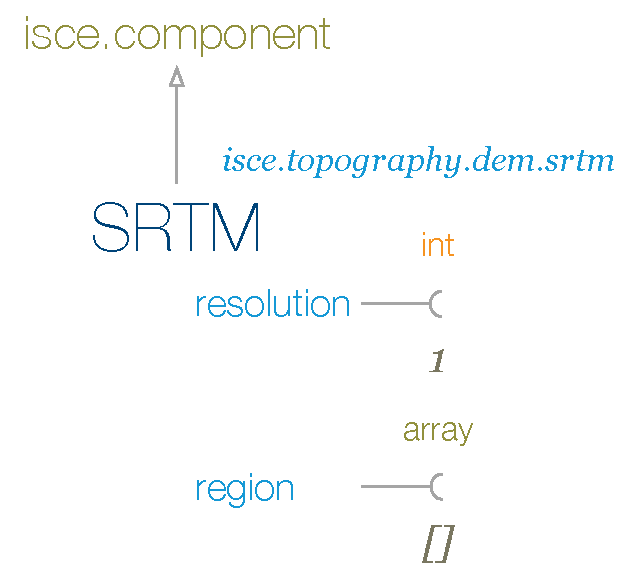
\includegraphics[height=20ex]{srtm-public}
    \end{center}
%
  \item prescribes the following modifications to \component{SRTM}
%
    \begin{ipython}[firstnumber=4, gobble=6]{}
      # the srtm component
      class SRTM(isce.component, family='isce.topography.dem.srtm'):
          """
          Access the SRTM data archive to download tiles and produce
          a digital elevation model for a specified region of interest
          """

          # user configurable state
          resolution = isce.properties.int(default=1)
          resolution.doc = 'the tile resolution in arc seconds per pixel'
          resolution.validators = isce.constraints.isMember(1, 3)

          region = isce.properties.array()
          region.doc = 'a cloud of (lat,lon) pairs'
    \end{ipython}
%
  \end{itemize}
%
\end{frame}

% --------------------------------------
\begin{frame}[fragile]
%
  \frametitle{Configuration --- \identifier{pfg}}
%
  \begin{itemize}
%
    \item \pyre\ loads configuration files whose name matches the name of a package automatically
%
    \item here is a sample configuration file in the native \identifier{pfg} format
%
      \begin{ipfg}[gobble=6]{}
        ; override the defaults in the component source code
        isce.topography.dem.srtm:
            region = [] ; empty, by default
            resolution = 1 ; arc seconds per pixel

        ; for an instance named la
        la:
            region = {regions.LA} ; a macro

        ; for an instance named greece
        greece:
            resolution = 3
            region = {regions.Greece}

        ; region aliases
        regions:
            LA = (33.3,-118.4), (35.7,-116.8)
            Greece = (41,26), (39,19), (34,24), (36,29)
      \end{ipfg}
%
    \item note that whitespace is significant: indentation captures the hierarchy
%
  \end{itemize}
%
\end{frame}

% --------------------------------------
\begin{frame}[fragile]
%
  \frametitle{Configuration --- \identifier{cfg}}
%
  \begin{itemize}
%
    \item here is the same configuration file in the alternative \identifier{cfg} format
%
      \begin{icfg}[gobble=6]{}
        ; override the defaults in the component source code
        [ isce.topography.dem.srtm ]
        region = [] ; empty, by default
        resolution = 1 ; arc seconds per pixel

        ; for an instance named la
        [ la ]
        region = {regions.LA}

        ; for an instance named greece
        [ greece ]
        resolution = 3
        region = {regions.Greece}

        ; region aliases
        [ regions ]
        LA = (33.3,-118.4), (35.7,-116.8)
        Greece = (41,26), (39,19), (34,24), (36,29)
      \end{icfg}
%
    \item no nesting
%
  \end{itemize}
%
\end{frame}

% --------------------------------------
\begin{frame}[fragile]
%
  \frametitle{Configuration --- \identifier{pml}}
%
  \begin{itemize}
%
    \item here is the same configuration file in the alternative \identifier{pml} format
%
      \begin{ipml}[gobble=6]{}
        <?xml version="1.0" encoding="utf-8"?>
        <config>
          <!-- override the defaults in the component source code -->
          <component family="isce.topography.dem.srtm">
            <bind property="region"> [] </bind>
            <bind property="resolution"> 1 </bind>
          </component>

          <!-- for an instance named la -->
          <component name="la">
            <bind property="region">{regions.LA}</bind>
          </component>

          <!-- for an instance named greece -->
          <component name="greece">
            <bind property="resolution">3</bind>
            <bind property="region">{regions.Greece}</bind>
            </component>

          <!-- region aliases -->
          <bind property="regions.LA">(33.3,-118.4), (35.7,-116.8)</bind>
          <bind property="regions.Greece">(41,26), (39,19), (34,24), (36,29)</bind>

        </config>
      \end{ipml}
%
  \end{itemize}
%
\end{frame}

% --------------------------------------
% recap
\begin{frame}
%
  \frametitle{Waypoint: components and their properties}
%
  \begin{itemize}
%
  \item \pyre\ components are evolved python objects
    \begin{itemize}
    \item the classes have family names, the instances get names when instantiated
    \item these names are unique strings in hierarchical namespaces delimited by periods
    \item collections of components form packages \emph{implicitly}, based on the topmost level
      in their namespace
    \end{itemize}
%
  \item components have properties that are under the control of the \emph{user}
    \begin{itemize}
    \item they look and behave like regular attributes
    \item they are \emph{typed} to enable conversions from strings
    \item they have default values and other metadata
    \end{itemize}
%
  \item configuration is partly about assigning values to component properties
    \begin{itemize}
    \item a requirement for supporting user interfaces
    \item intuitive syntax for the command line
    \item simple configuration files in a variety of formats:
      \begin{itemize}
      \item \identifier{pfg}: the preferred native format
      \item \identifier{pml}: an \identifier{XML} dialect
      \item \identifier{cfg}: a format inspired by the Microsoft Windows \identifier{.ini} format
      \end{itemize}
    \end{itemize}
%
  \item configuration is automatically handled by the framework and requires no explicit
    involvement on the part of the component author
%
  \end{itemize}
%
\end{frame}

%-----------------------------------
\begin{frame}
%
  \frametitle{Waypoint: notation for components and their properties}
%
    \only<1>{
      \begin{center}
        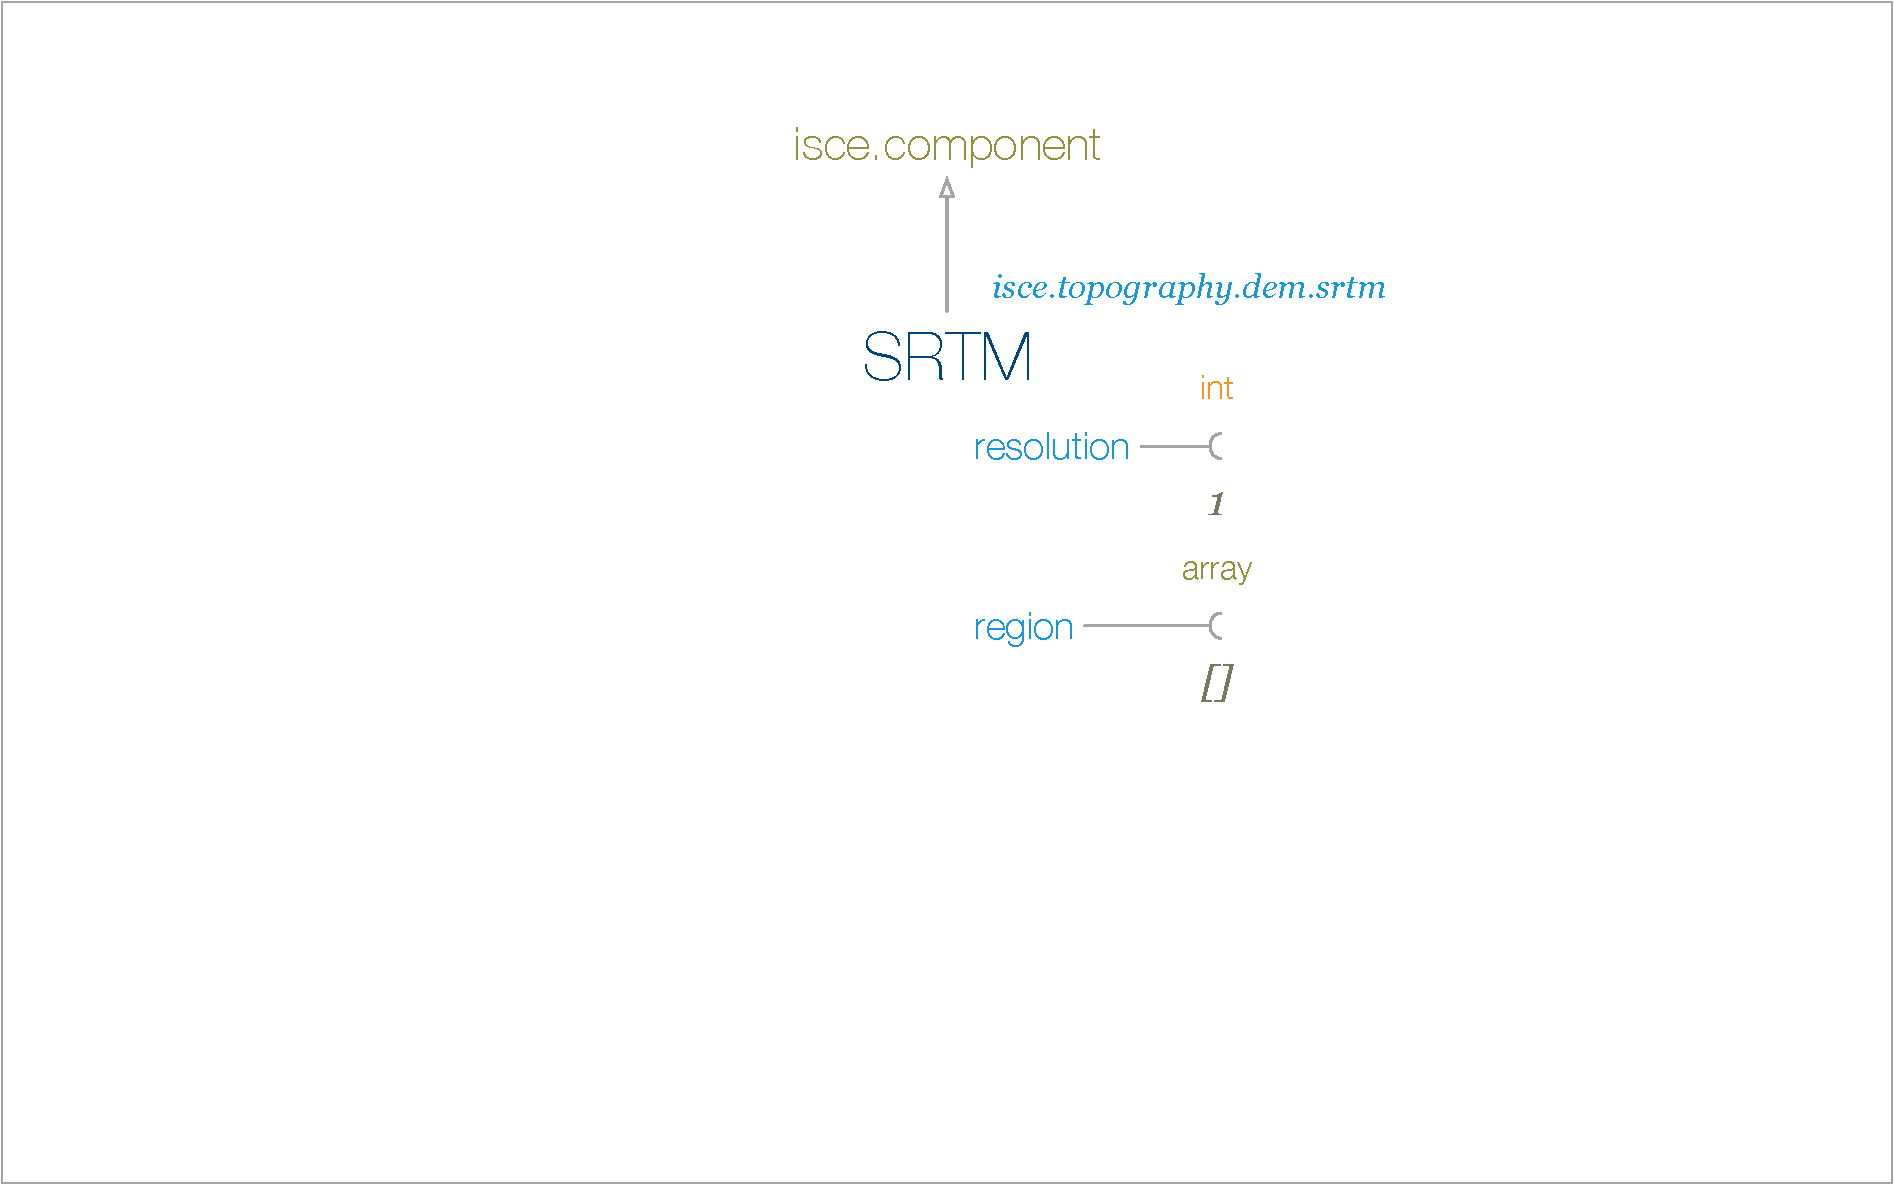
\includegraphics[width=0.9\textwidth]{component-wayprop-class}
      \end{center}
    }
    \only<2>{
      \begin{center}
        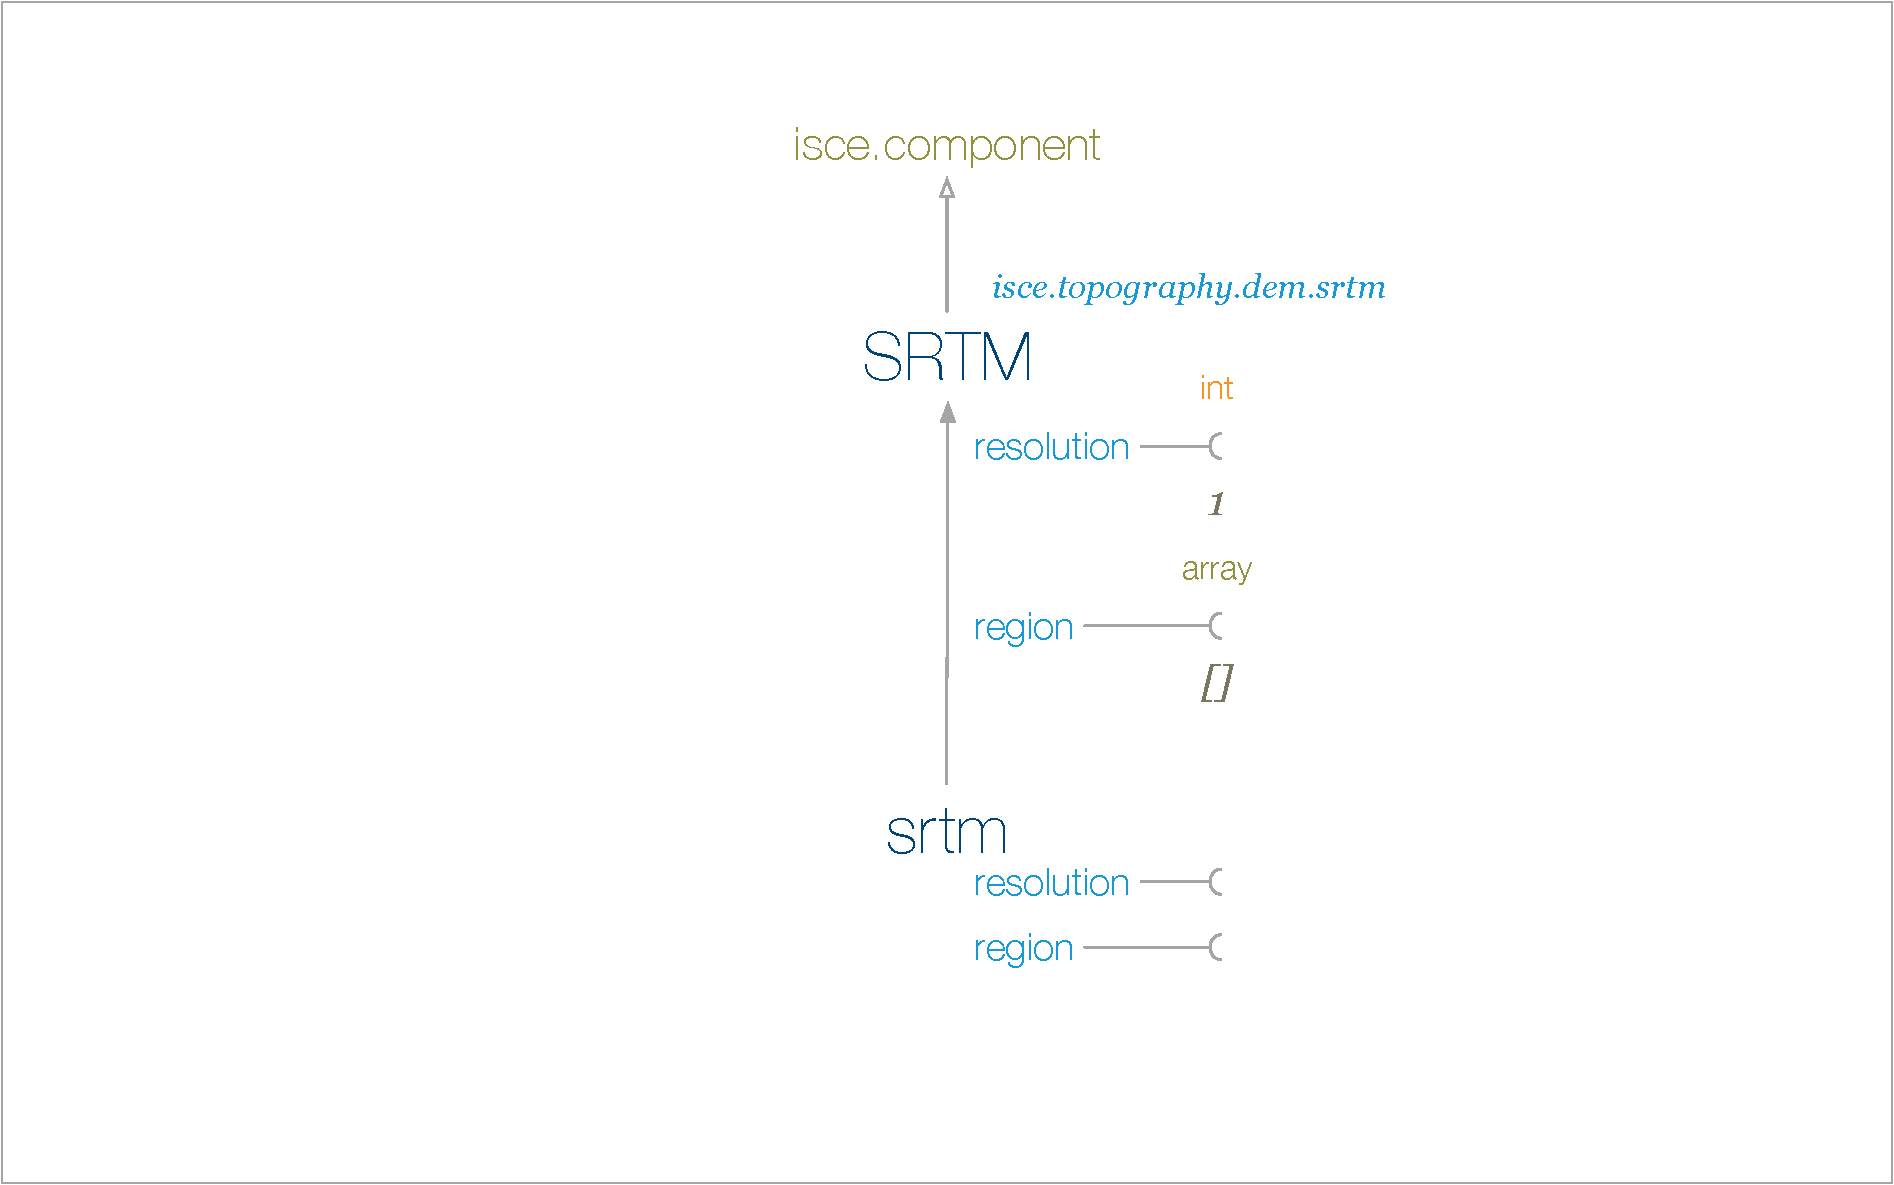
\includegraphics[width=0.9\textwidth]{component-wayprop-instance}
      \end{center}
    }
%
\end{frame}

% --------------------------------------
\subsection{behaviors}

\begin{frame}[fragile]
%
  \frametitle{Behaviors}
%
  \vskip -3ex
  \begin{itemize}
%
    \item Component methods may be marked public
%
      \begin{ipython}[firstnumber=4, gobble=6]{}
        # the srtm component
        class SRTM(isce.component, family='isce.topography.dem.srtm'):
  \end{ipython}
%
  \item here is what \component{SRTM} can do:
%
  \begin{ipython}[firstnumber=19, gobble=6]{}
           @isce.export
           def authenticate(self, ...):
               """
               Retrieve and store the user's authentication credentials
               """

            @isce.export
            def plan(self, ...):
                """
                Describe the work required to generate the specified DEM
                """

            @isce.export
            def download(self, ...):
                """
                Retrieve the tiles necessary to cover the convex hull of my {region}
                """

            @isce.export
            def stitch(self, ...):
                """
                Assemble the elevation model
                """
    \end{ipython}
%
  \end{itemize}
%
\end{frame}

% --------------------------------------
\begin{frame}
%
  \frametitle{}
%
\end{frame}

% --------------------------------------
\subsection{protocols}
\begin{frame}
%
  \frametitle{Wiring components to each other}
%
  \begin{itemize}
%
  \item the real power of the framework is in letting components be properties,
    i.e.~configurable state, for other components
%
  \item imagine
    \begin{itemize}
    \item a component \component{Topo} that needs a \dem\ of a given region
    \item multiple implementations of components that can stitch {\dem}s together
    \end{itemize}
%
  \item it is natural to want to let the user pick among the alternative implementations and
    take control of the wiring; we need
%
    \begin{itemize}
    \item a way for \component{Topo} to express that it \emph{requires} a \dem\
      stitcher
    \item to express that \component{SRTM} and its alternatives can \emph{satisfy} this
      requirement
    \item a way for the end user to specify which alternative she prefers
    \item a way for the framework to locate, instantiate, and validate the user's choice
    \end{itemize}
%
  \item we must be able to translate strings to configured component instances
%
  \item upon reflection, the process is very similar to our treatment of the simpler types
%
  \end{itemize}
%
\end{frame}

% --------------------------------------
\begin{frame}
%
  \frametitle{Components and protocols}
%
  \begin{itemize}
%
  \item let's separate expressing the requirement from satisfying it
      \begin{itemize}
      \item \emph{protocols} are abstract specifications of application requirements
      \item \emph{components} are concrete implementations that satisfy requirements
      \end{itemize}
%
    \item protocols make it possible to write applications without any \emph{a priori} knowledge
      of implementation specifics
%
    \item inversion of control\supercite{johnson-88}:
      \begin{itemize}
      \item a design pattern\supercite{patterns} that enables the assembly of applications out
        of interchangeable parts, under the control of the end user
      \item the selection and binding of actual implementations to the application requirements
        happens at runtime
      \end{itemize}
%
    \item in \pyre, the user
      \begin{itemize}
      \item controls the application state through configuration files, the user interface, the
        command line
      \item specifies components using simple URIs
      \end{itemize}
%
    \item the goal is to isolate contributors from each other as much as possible, and provide
      a coherent and usable strategy for composing non-trivial applications
%
  \end{itemize}
%
\end{frame}

%-----------------------------------
\begin{frame}
%
  \frametitle{Indicating the protocol}
%
  \only<1>{
    \begin{center}
      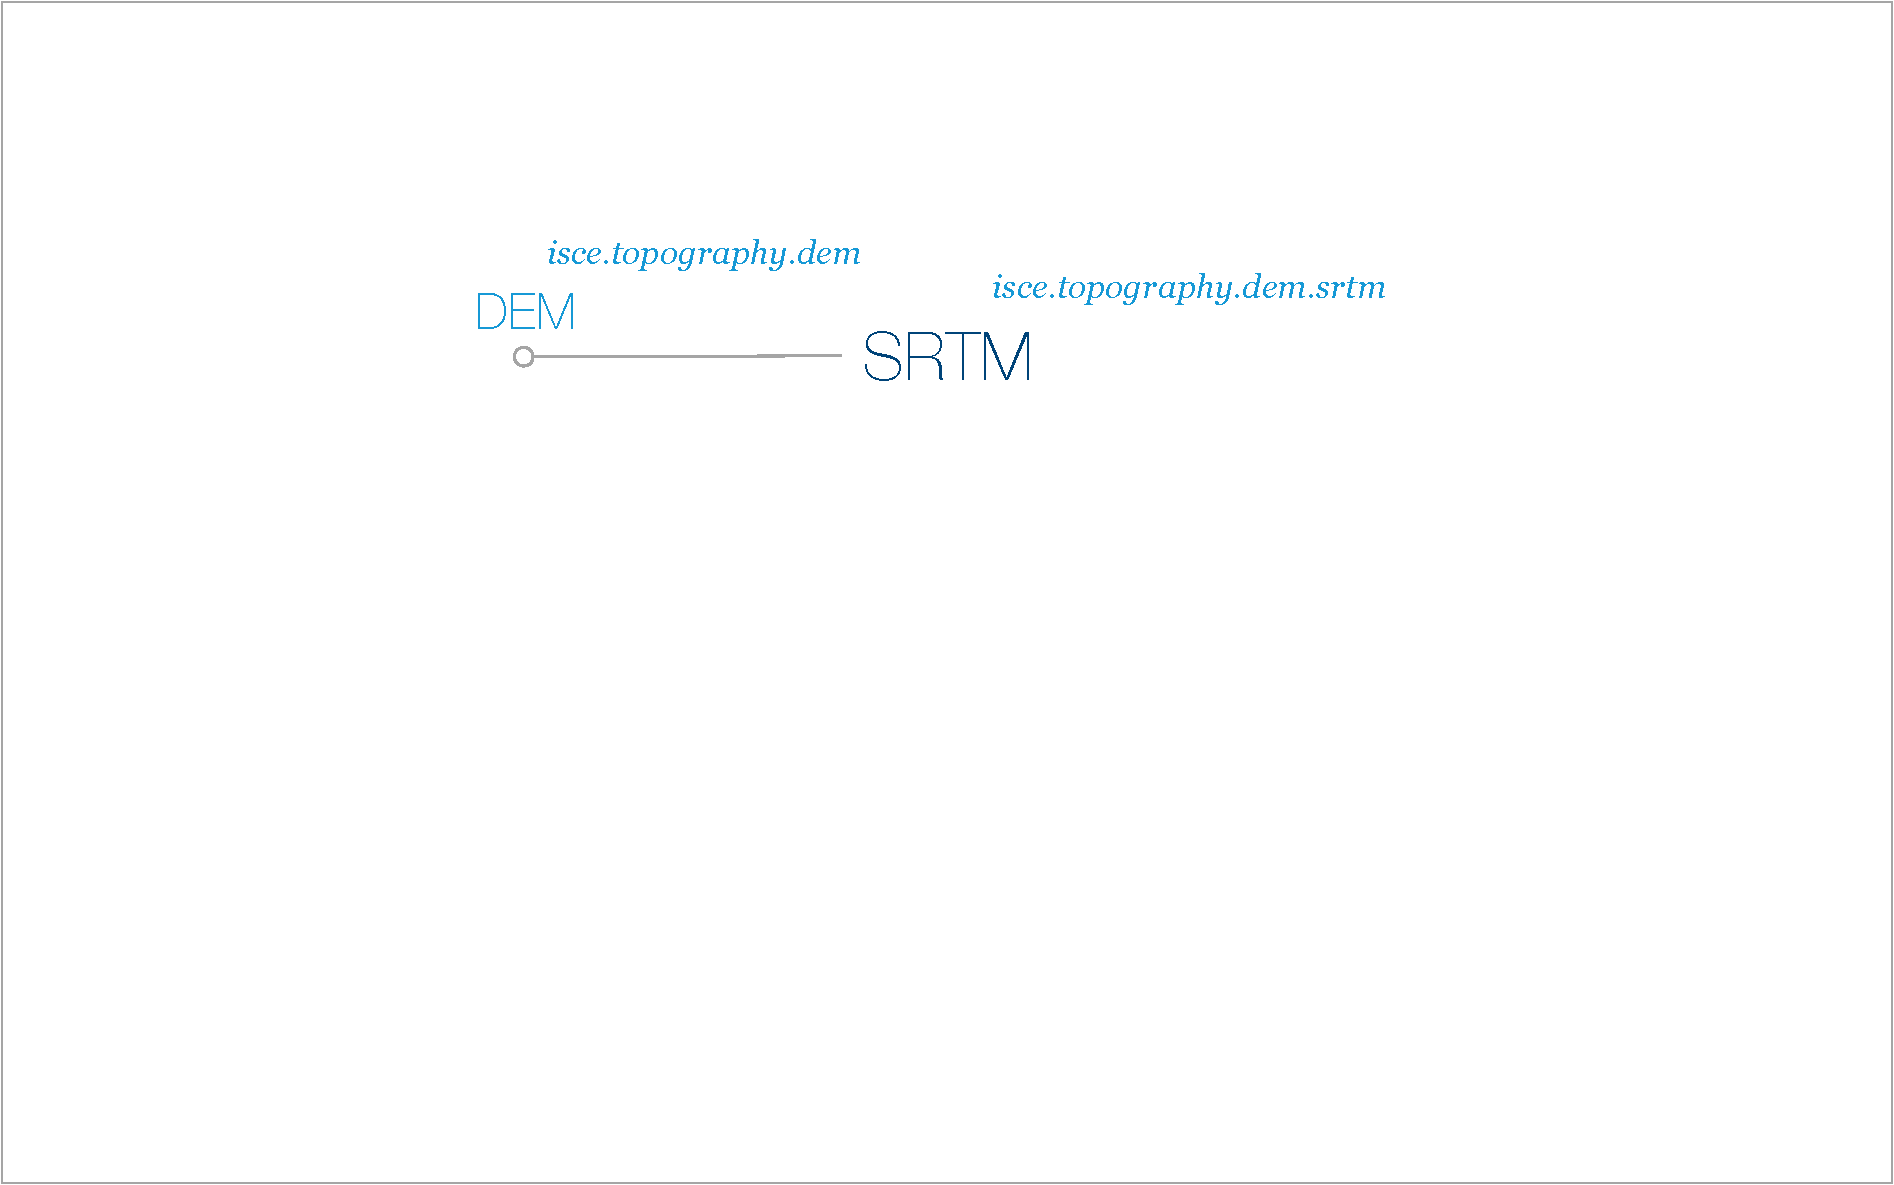
\includegraphics[width=0.9\textwidth]{component-implements}
    \end{center}
  }
  \only<2>{
    \begin{center}
      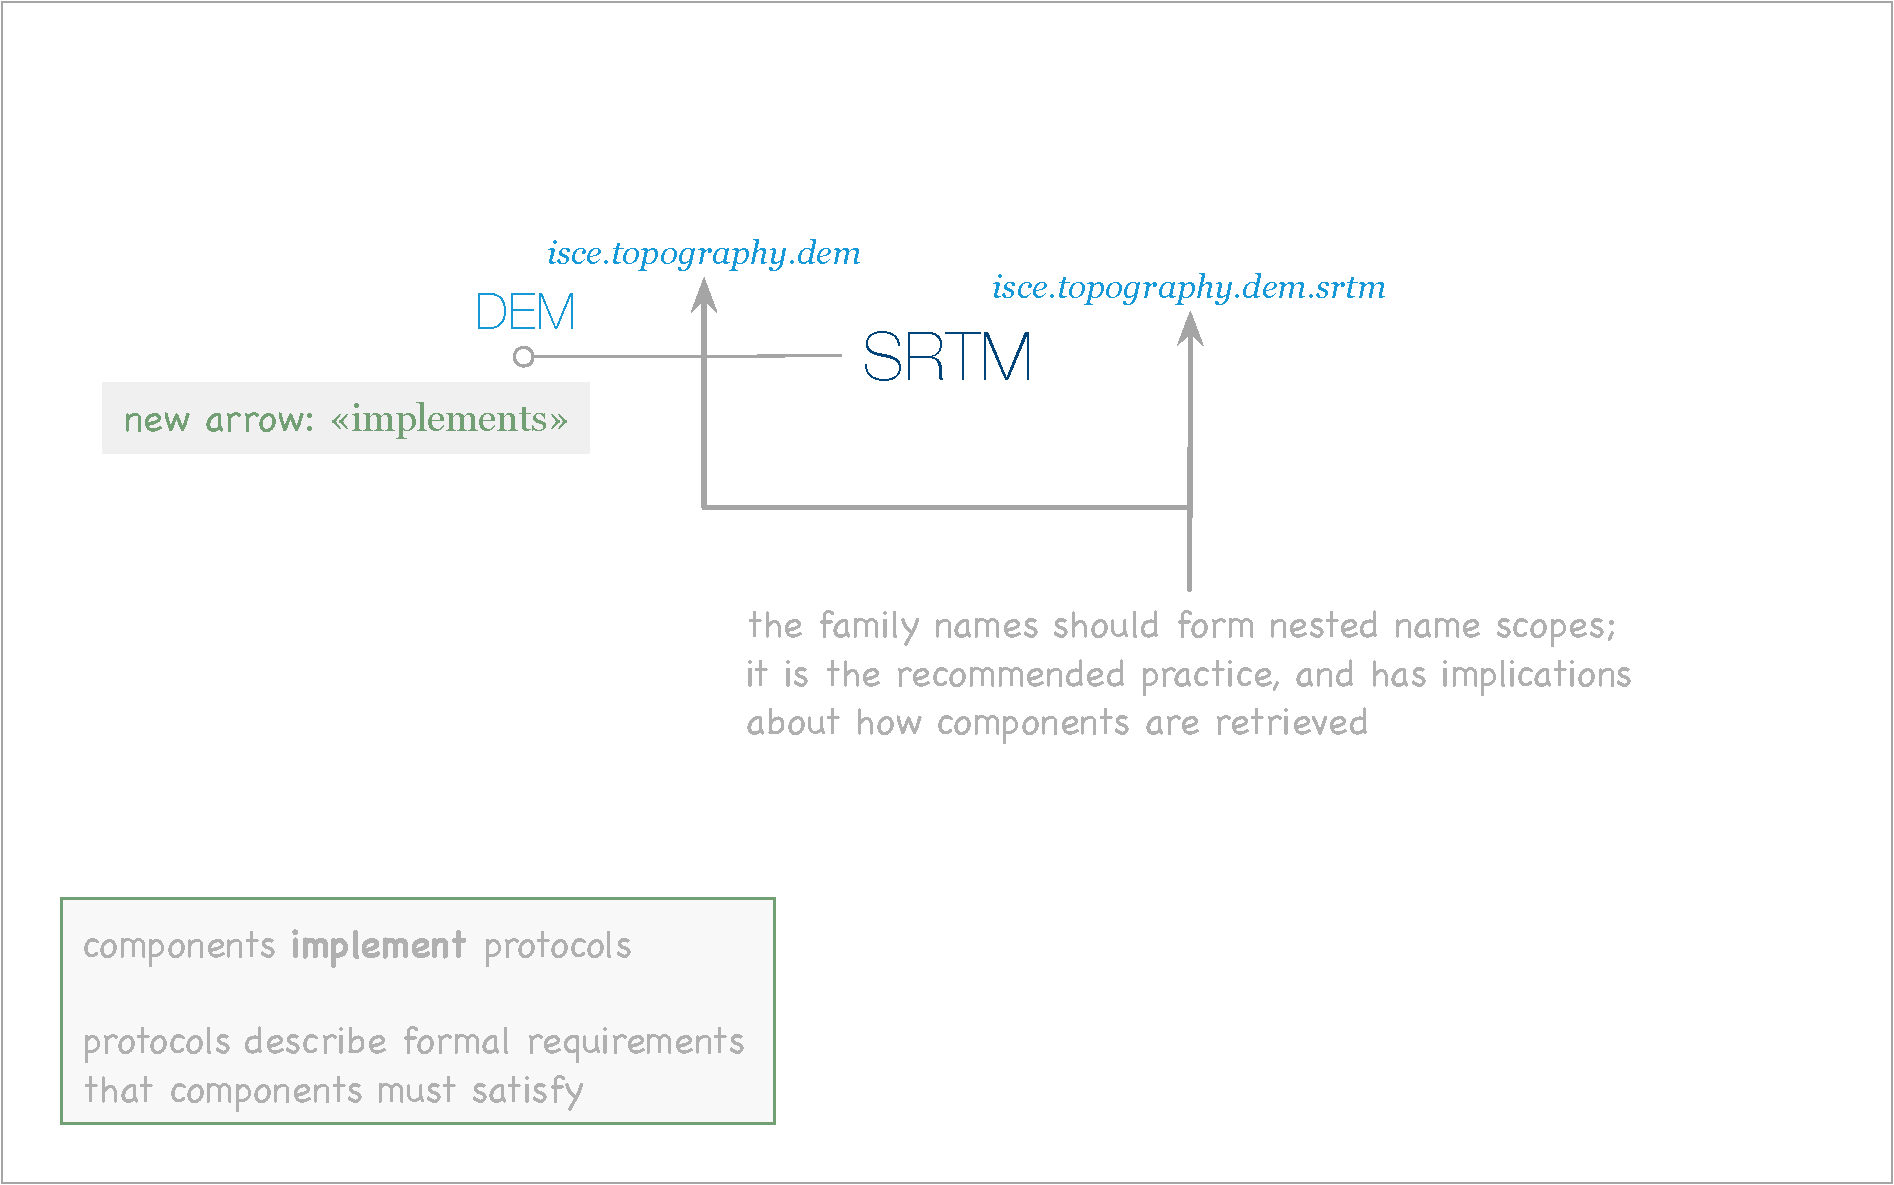
\includegraphics[width=0.9\textwidth]{component-implements-explained}
    \end{center}
  }
  \only<3>{
    \begin{center}
      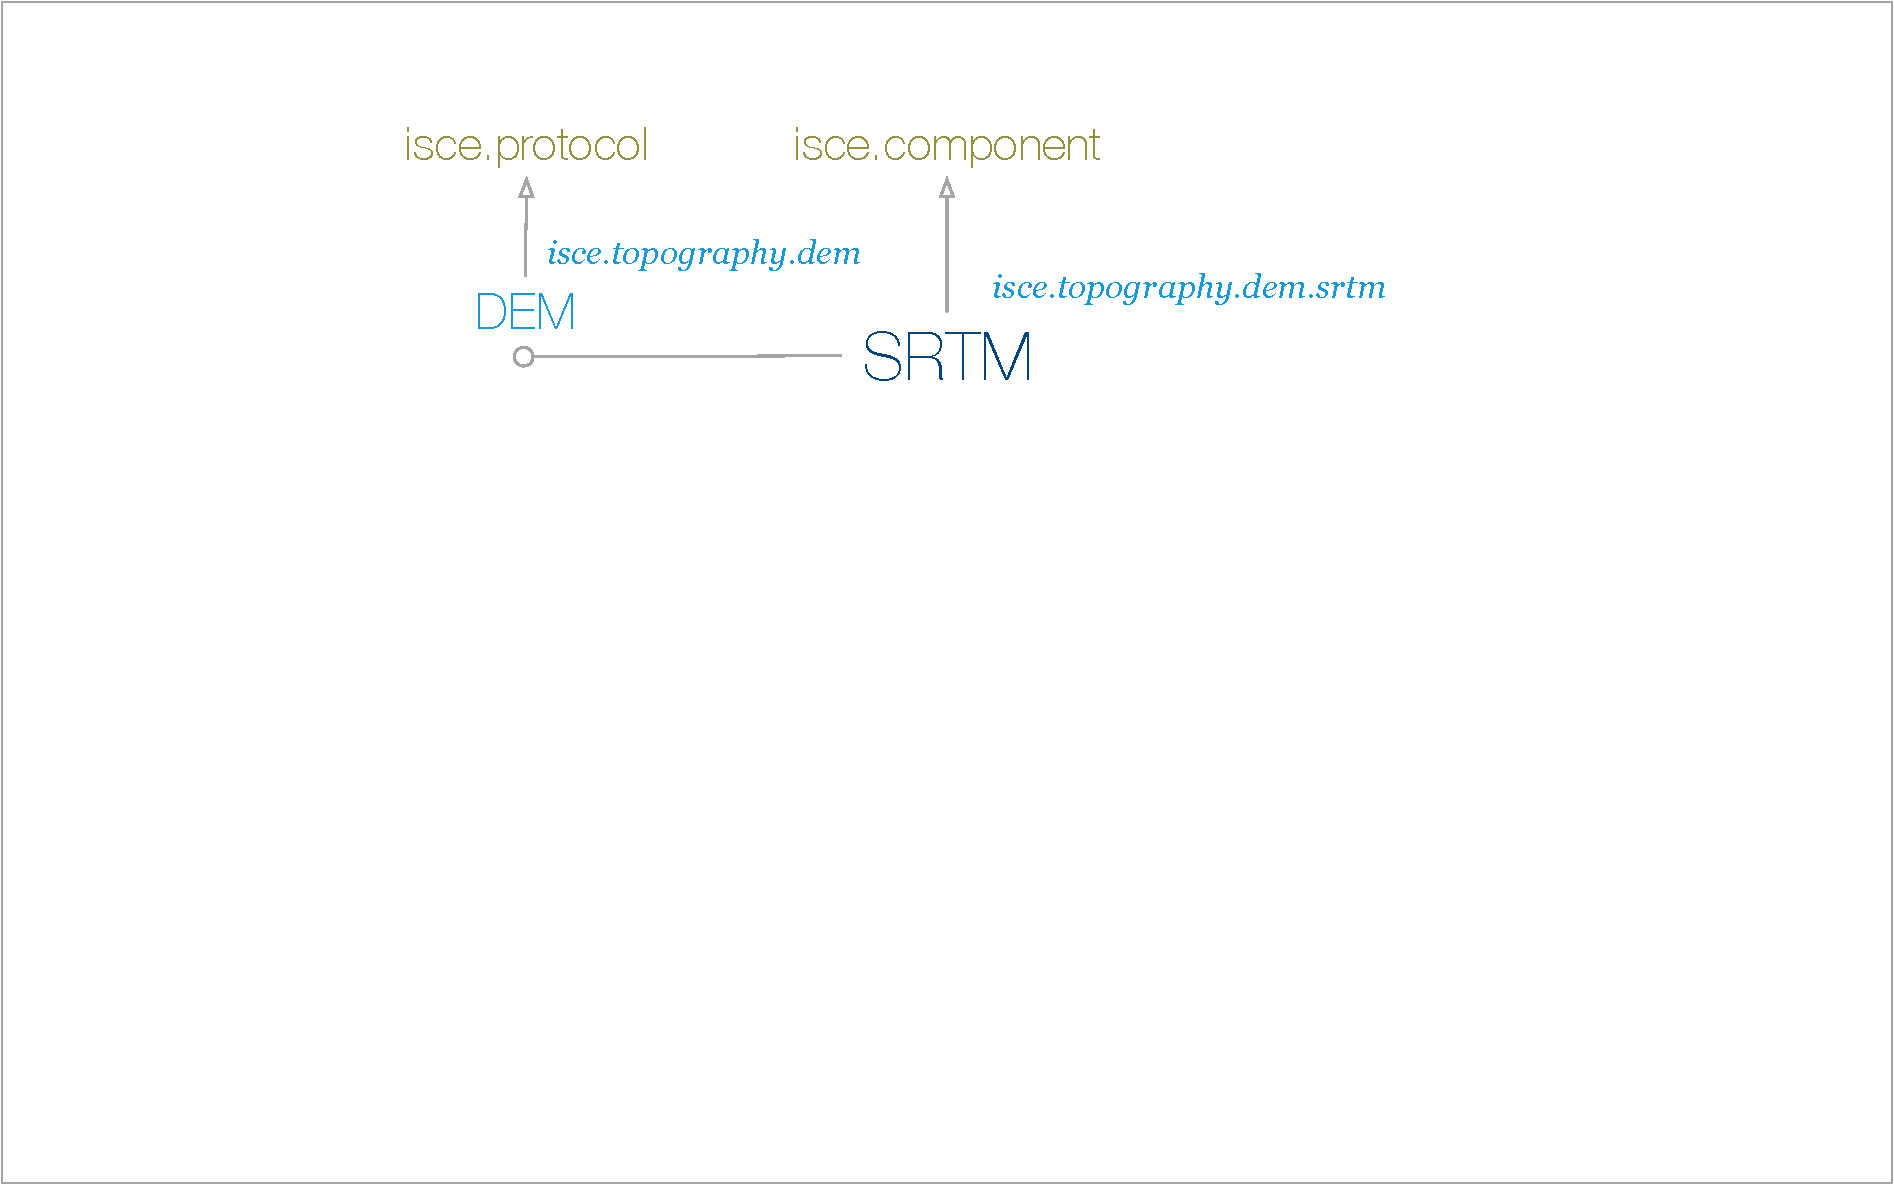
\includegraphics[width=0.9\textwidth]{component-implements-pedigree}
    \end{center}
  }
%
\end{frame}

% --------------------------------------
\begin{frame}[fragile]
%
  \frametitle{Protocol declaration}
%
  \vskip -3ex
  \begin{itemize}
%
  \item the \protocol{DEM} declaration is very similar to the declaration of \component{SRTM}
%
  \item the design decision to be made here is what should one require of \emph{all}
    \protocol{DEM} implementors, regardless of their implementation details
%
      \begin{ipython}[firstnumber=4, gobble=6]{}
        # the srtm component
        class DEM(isce.protocol, family='isce.topography.dem'):
            """
            Requirements for components that assemble digital elevation models
            """

            # user configurable state
            region = isce.properties.array()
            region.doc = 'the specification of the region of interest'

            # required behavior
            @isce.provides
            def plan(self, ...):
                """
                Describe the work required to generate the specified DEM
                """

            @isce.provides
            def stitch(self, ...):
                """
                Assemble the elevation model
                """
    \end{ipython}
%
  \item it makes sense to not only require behavior, but configurable state as well, since both
    are part of the public interface
%
  \end{itemize}
%
\end{frame}

% --------------------------------------
\begin{frame}
%
  \frametitle{A sneak peak at \pyre\ internals}
%
  \vskip -3ex
  \begin{center}
    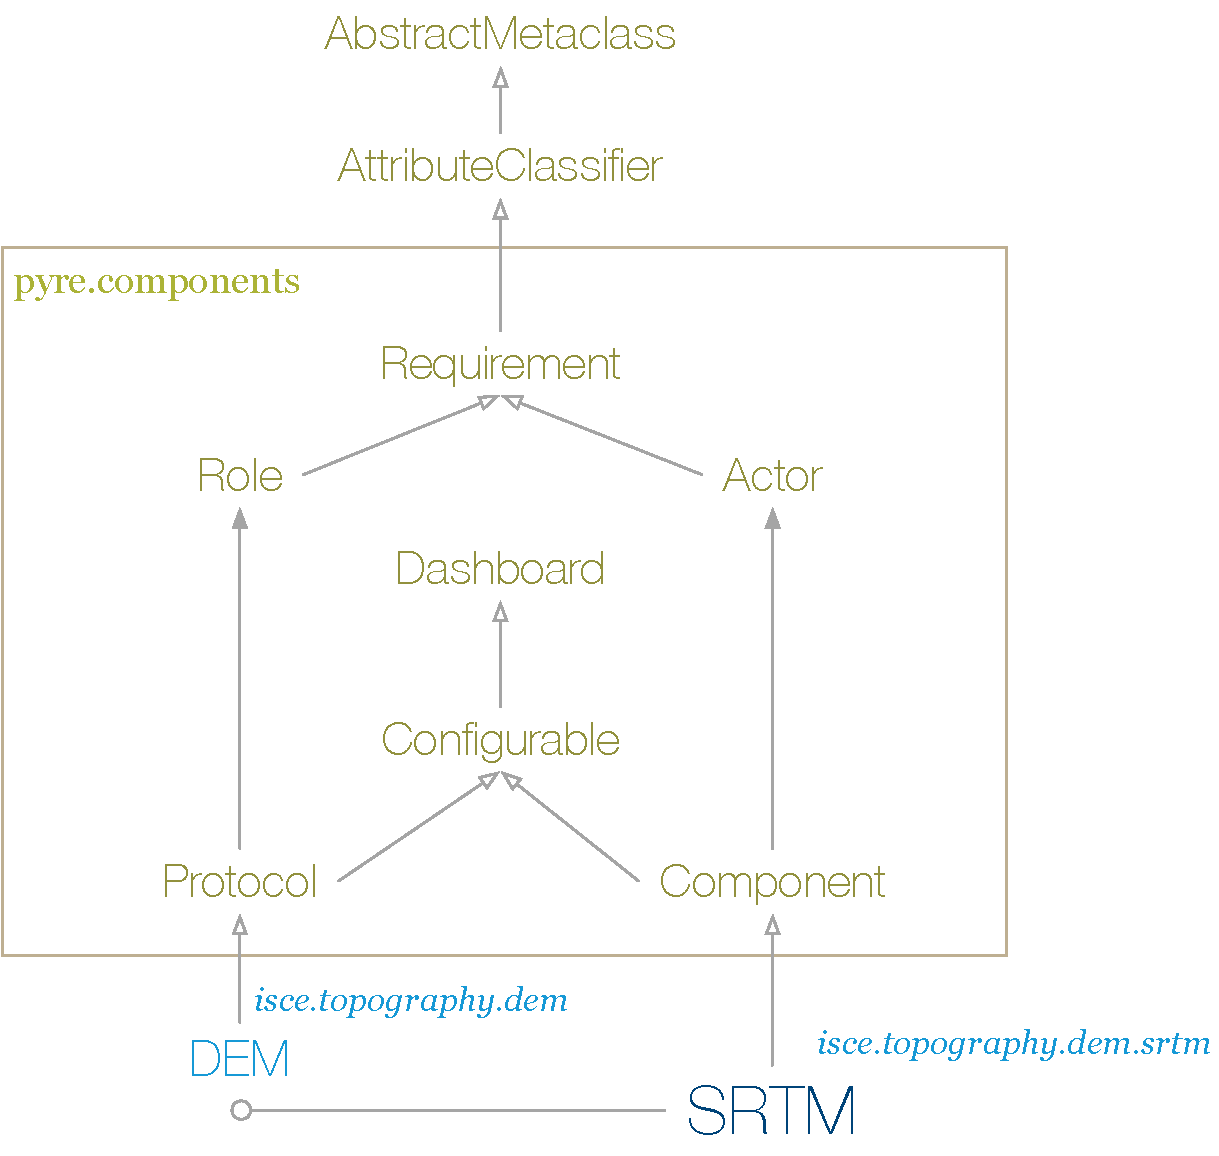
\includegraphics[height=0.8\textheight]{pyre-configurables}
  \end{center}
%
\end{frame}

% --------------------------------------
\begin{frame}[fragile]
%
  \frametitle{Specifying the protocol in the component declaration}
%
  \vskip -3ex
  \begin{itemize}
%
  \item the instruction
%
    \begin{center}
      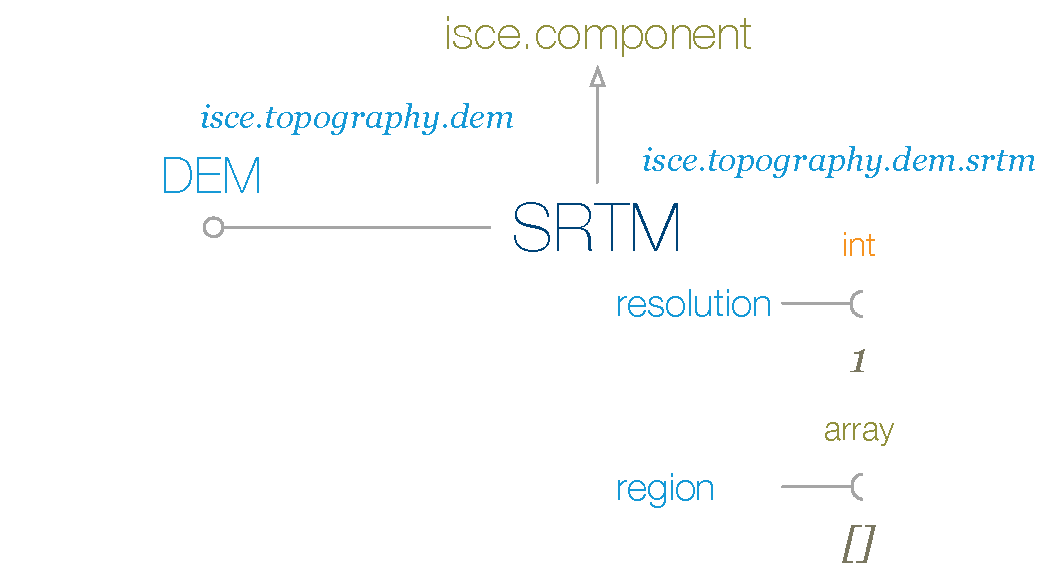
\includegraphics[height=20ex]{srtm-implements}
    \end{center}
%
  \item prescribes the following modification to the declaration of \component{SRTM}
%
    \begin{ipython}[firstnumber=4, gobble=6]{}
      # the srtm component
      class SRTM(isce.component, family='isce.topography.dem.srtm',
                  implements=isce.topography.dem):
          """
          Access the SRTM data archive to download tiles and produce
          a digital elevation model for a specified region of interest
          """
    \end{ipython}
%
    assuming that the package \package{isce.topography} correctly encapsulates the class
    \class{DEM} in the symbol \identifier{dem} by a correctly structured \keyword{import}
    statement
%
  \item the framework checks compliance at compile time, i.e the first time the
    \package{SRTM.py} is imported
%
  \item proper namespace design simplifies how the user selects an actual implementation
    \begin{itemize}
      \item by enabling intuitive shorthand
      \item more on this later
    \end{itemize}
%
  \end{itemize}
%
\end{frame}

%-----------------------------------
\begin{frame}
%
  \frametitle{Fully decorated component}
%
  \only<1>{
    \begin{center}
      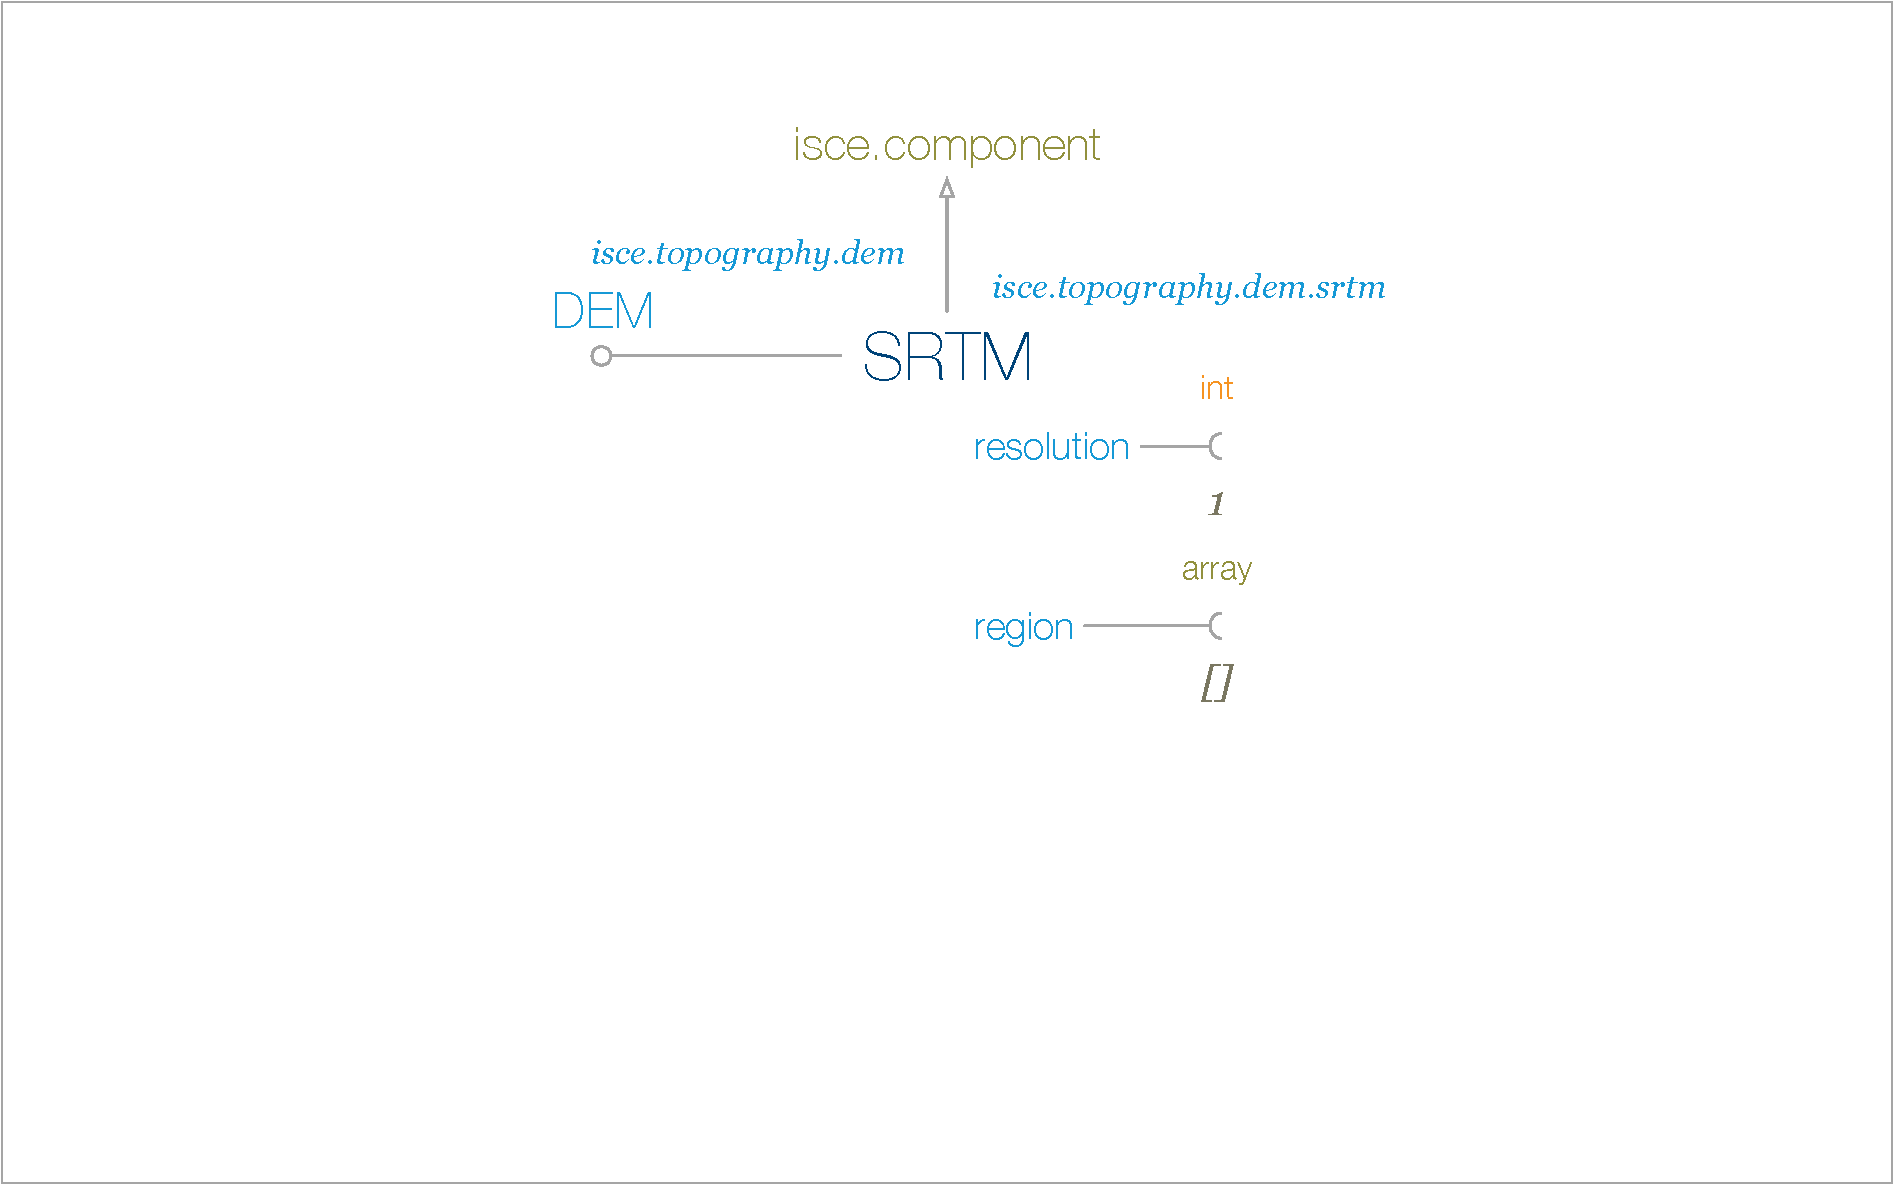
\includegraphics[width=0.9\textwidth]{component-decorated}
    \end{center}
  }
%
  \only<2>{
    \begin{center}
      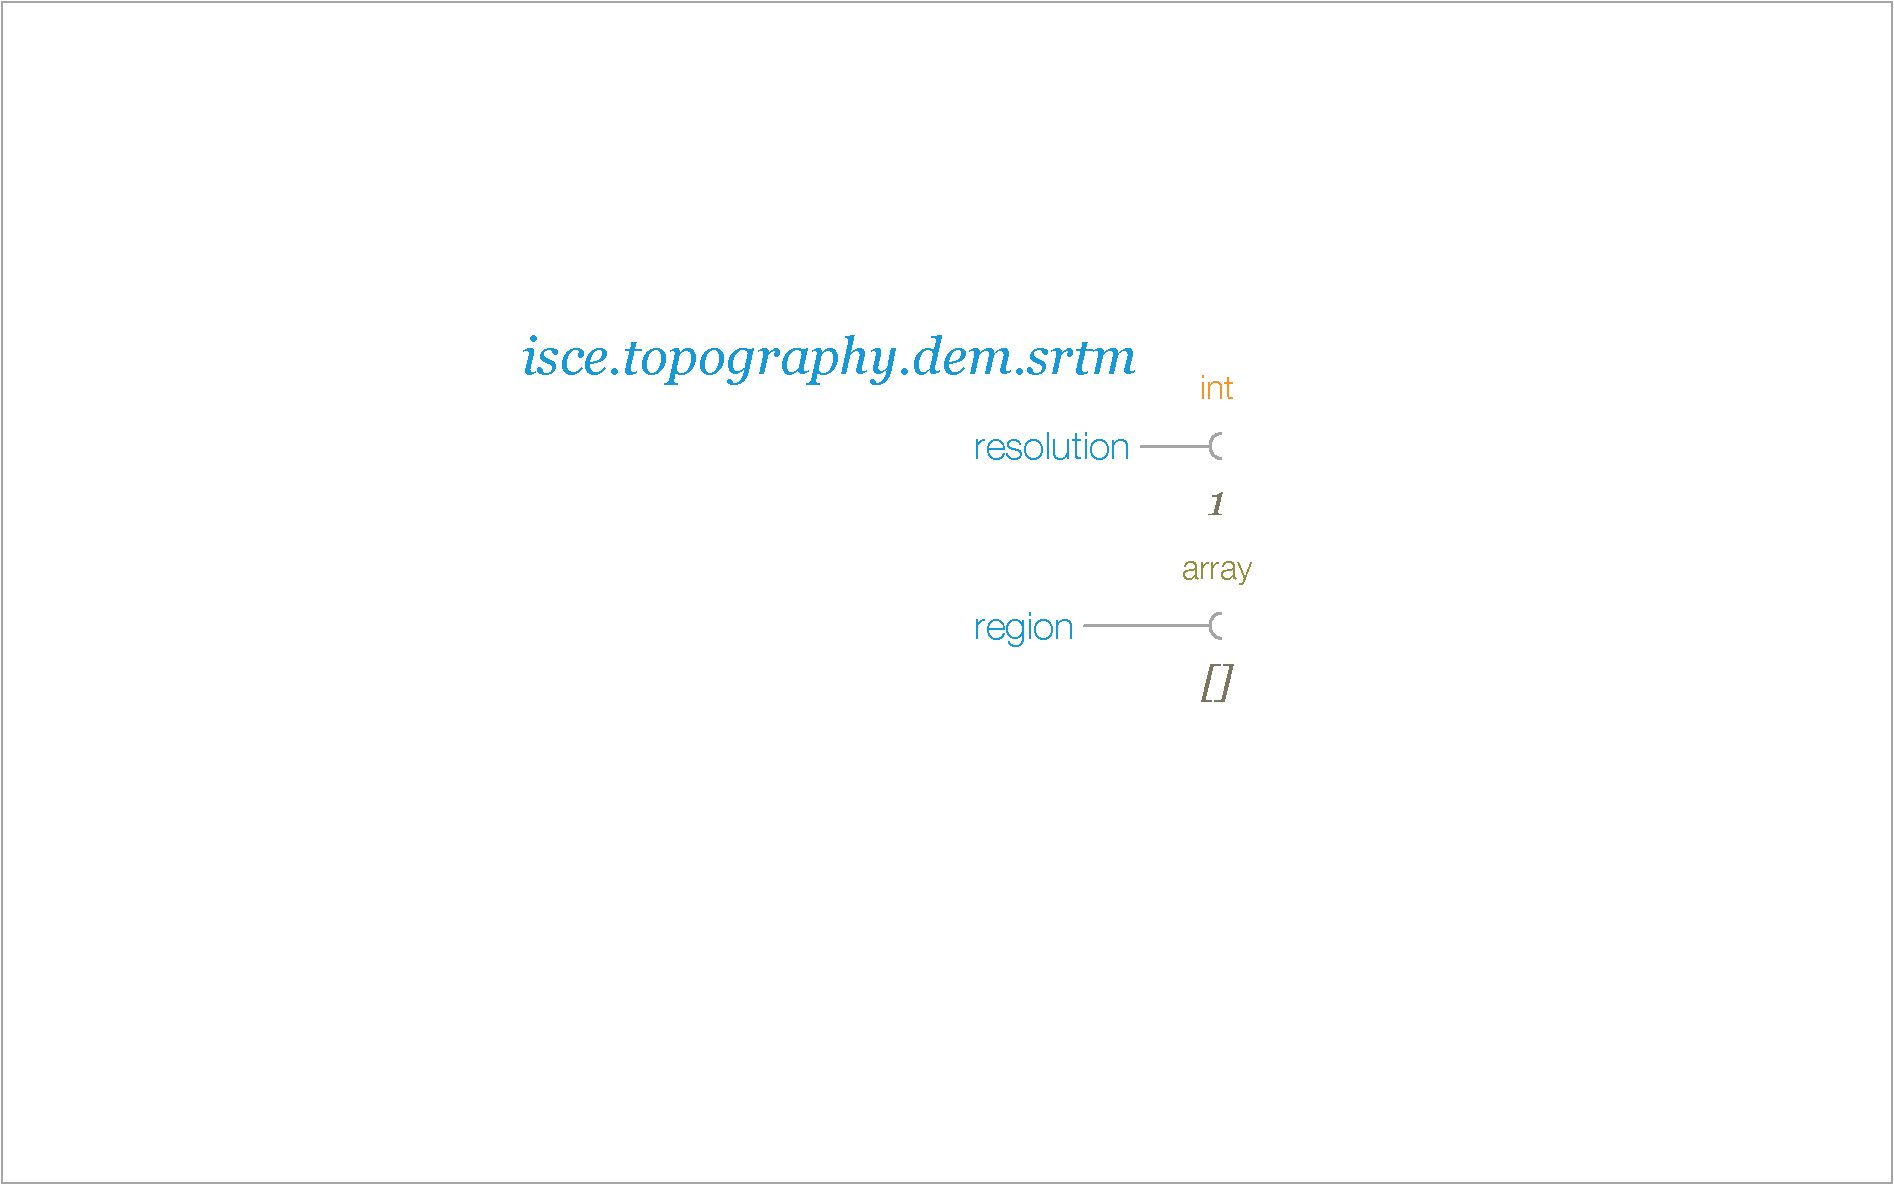
\includegraphics[width=0.9\textwidth]{component-decorated-config}
    \end{center}
  }
%
\end{frame}

% --------------------------------------

\TODO{
  \item properties
    \begin{itemize}
    \item point out the '.'join(...) structure of names, which mimics python scopes
    \item explain conditional assignments
    \item syntax rules for each format
    \item explain which files are loaded automatically
    \item explain how \pyre\ looks for configuration files
    \item explain priorities
    \item
    \end{itemize}
%
  \item behaviors
%
  \item protocols
}

%%% Local Variables:
%%% mode: latex
%%% TeX-master: "../pyre"
%%% End:

% end of file
